%% This is the ctufit-thesis example file. It is used to produce theses
%% for submission to Czech Technical University, Faculty of Information Technology.
%%
%% This is version 1.4.3, built 1. 4. 2025.
%% 
%% Get the newest version from
%% https://gitlab.fit.cvut.cz/theses-templates/FITthesis-LaTeX
%%
%%
%% Copyright 2024, Tomas Novacek
%% Copyright 2021, Eliska Sestakova and Ondrej Guth
%%
%% This work may be distributed and/or modified under the
%% conditions of the LaTeX Project Public License, either version 1.3
%% of this license or (at your option) any later version.
%% The latest version of this license is in
%%  https://www.latex-project.org/lppl.txt
%% and version 1.3 or later is part of all distributions of LaTeX
%% version 2005/12/01 or later.
%%
%% This work has the LPPL maintenance status `maintained'.
%%
%% The current maintainer of this work is Tomas Novacek (novacto3@fit.cvut.cz).
%% Alternatively, submit bug reports to the tracker at
%% https://gitlab.fit.cvut.cz/theses-templates/FITthesis-LaTeX/issues
%%
%%

% arara: xelatex
% arara: biber
% arara: xelatex
% arara: xelatex

%%%%%%%%%%%%%%%%%%%%%%%%%%%%%%%%%%%%%%%%%
% CLASS OPTIONS
% language: czech/english/slovak
% thesis type: bachelor/master/dissertation
% colour: bw for black&white OR no option for default colour scheme
% electronic (oneside) or printed (twoside), twoside is default
% paragraph - if passed, this optional argument sets paragraphs as the deepest level of headers, styles it, numbers it and adds it to Table of Content. Use with care! Normally, it is considered unwise to use it, since its too deep.
%%%%%%%%%%%%%%%%%%%%%%%%%%%%%%%%%%%%%%%%%
\documentclass[english,bachelor,oneside]{ctufit-thesis} % WHEN CHANGING ONESIDE-TWOSIDE, ALSO CHANGE CLEARPAGE BEFORE NUMBERED CHAPTERS

%%%%%%%%%%%%%%%%%%%%%%%%%%%%%%%%%%
% FILL IN THIS INFORMATION
%%%%%%%%%%%%%%%%%%%%%%%%%%%%%%%%%%
\ctufittitle{Grafit.games - Commercialization of Student Game Projects} % replace with the title of your thesis
\ctufitauthorfull{Samuel Černák} % replace with your full name (first name(s) and then family name(s) / surname(s)) including academic degrees
\ctufitauthorsurnames{Černák} % replace with your surname(s) / family name(s)
\ctufitauthorgivennames{Samuel} % replace with your first name(s) / given name(s)
\ctufitsupervisor{Bc. Ondřej Brém\, MSc.} % replace with name of your supervisor/advisor (include academic degrees)
\ctufitdepartment{Department of Software Engineering} % replace with the department of your defence
\ctufityear{2025} % replace with the year of your defence
\ctufitdeclarationplace{Prague} % replace with the place where you sign the declaration
\ctufitdeclarationdate{May 13, 2025} % replace with the date of signature of the declaration
\ctufitabstractCZE{Tato práce zkoumá, proč jsou hry vytvářené studenty na FITu po dokončení často opuštěny, a hledá řešení tohoto problému. Přestože v Praze objem soukromých investic roste, studentské podnikání zůstává na nízké úrovni. Naše fakulta postrádá mechanismus na podporu komercializace herních projektů. Navrh jsem systém, který motivuje k dalšímu rozvoji těchto projektů. V rešerši se zabývám procesem vývoje her, existující institucionální podporou v jiných prostředích a možnými způsoby vstupu na trh. Na základě těchto zjištění jsem navrh systém založený na principu družstva, přizpůsoben potřebám studentů. V rámci práce jsem spustili náborový web, začal sbírat kontakty a názory od potenciálních účastníků a připravil testovací mechanismus. Přestože nebyla zřízena žádná právnická osoba, poskytuji návrh stanov a návod k založení. Tato práce tak vytváří základ pro udržitelnou podpůrnou strukturu, která může studentům pomoci rozvinout podnikatelský potenciál jejich tvůrčích projektů.}
\ctufitabstractENG{This thesis explores why student-created games at FIT are often abandoned after completion and proposes a solution. Despite increasing private investment in Prague, student entrepreneurship remains low—partly due to the lack of institutional mechanisms supporting the commercialization of student projects. I propose a system that encourages further development and potential market entry of student-made games. In the research I examine the game development process, examples of institutional support elsewhere, and possible commercialization pathways. Based on these insights I present a lightweight cooperative-based framework tailored to students’ needs. As part of the thesis, I launched a recruitment website, started collecting contacts and feedback from potential participants, and designed a testing mechanism. While no legal entity was established, statutes and a funding guide are provided. Ultimately, the work lays a foundation for a sustainable support structure that can empower students to pursue the entrepreneurial potential of their creative projects.}
\ctufitkeywordsCZE{vývoj her, uvedení hry na trh, podpora studentů, podpůrný mechanismus, podpůrný program, vedené studenty, start-up, duševní vlastnictví, licence, univerzitní inkubátor}
\ctufitkeywordsENG{game development, game launch, student support, support mechanism, support programme, student-led, start-up, intellectual property, licensing, university incubator}
%%%%%%%%%%%%%%%%%%%%%%%%%%%%%%%%%%
% END FILL IN
%%%%%%%%%%%%%%%%%%%%%%%%%%%%%%%%%%

%%%%%%%%%%%%%%%%%%%%%%%%%%%%%%%%%%
% CUSTOMIZATION of this template
% Skip this part or alter it if you know what you are doing.
%%%%%%%%%%%%%%%%%%%%%%%%%%%%%%%%%%
\setlength{\parindent}{0pt}                        % Remove paragraph indentation
\setlength{\parskip}{0.5em plus 0.1em minus 0.1em}  % Add vertical space between paragraphs
\setlength{\belowcaptionskip}{6pt}

\RequirePackage{iftex}[2020/03/06]
\iftutex % XeLaTeX and LuaLaTeX
    \RequirePackage{ellipsis}[2020/05/22] %ellipsis workaround for XeLaTeX
\else
    \errmessage{Only compilation with XeLaTeX or LuaLaTeX is allowed}
    \stop
\fi

% hyperlinks
\hypersetup{
    pdfpagelayout=TwoPageRight,
    colorlinks=false,
    allcolors=decoration,
    pdfborder={0 0 0.1}
}

% uncomment the following to hide all hyperlinks
%\hypersetup{hidelinks}

% uncomment the following to change the colour of all hyperlinks to CTU blue
%\hypersetup{allbordercolors=decoration}

\RequirePackage{pdfpages}[2020/01/28]

%%%%%%%%%%%%%%%%%%%%%%%%%%%%%%%%%%
% CUSTOMIZATION of this template END
%%%%%%%%%%%%%%%%%%%%%%%%%%%%%%%%%%


%%%%%%%%%%%%%%%%%%%%%%
% PACKAGES SETTINGS
% You may choose to modify this part.
%%%%%%%%%%%%%%%%%%%%%%
\usepackage{dirtree}
\usepackage{lipsum,tikz}
\usepackage[style=iso-numeric]{biblatex}
\addbibresource{text/bib-database.bib}
\usepackage{xurl}
\usepackage{listings} % typesetting of sources
%\usepackage{minted}
\usepackage{csquotes}
\usepackage{float}
\graphicspath{{images/}}
% \graphicspath{{appeded/posters/}}
\usepackage{xr-hyper}
\usepackage{enumitem}

%%%%%%%%%%%%%%%%%%%%%%
% PACKAGES SETTINGS END
%%%%%%%%%%%%%%%%%%%%%%

\begin{document} 
\frontmatter\frontmatterinit % do not remove these two commands

\thispagestyle{empty}\maketitle\thispagestyle{empty}\cleardoublepage % do not remove these four commands

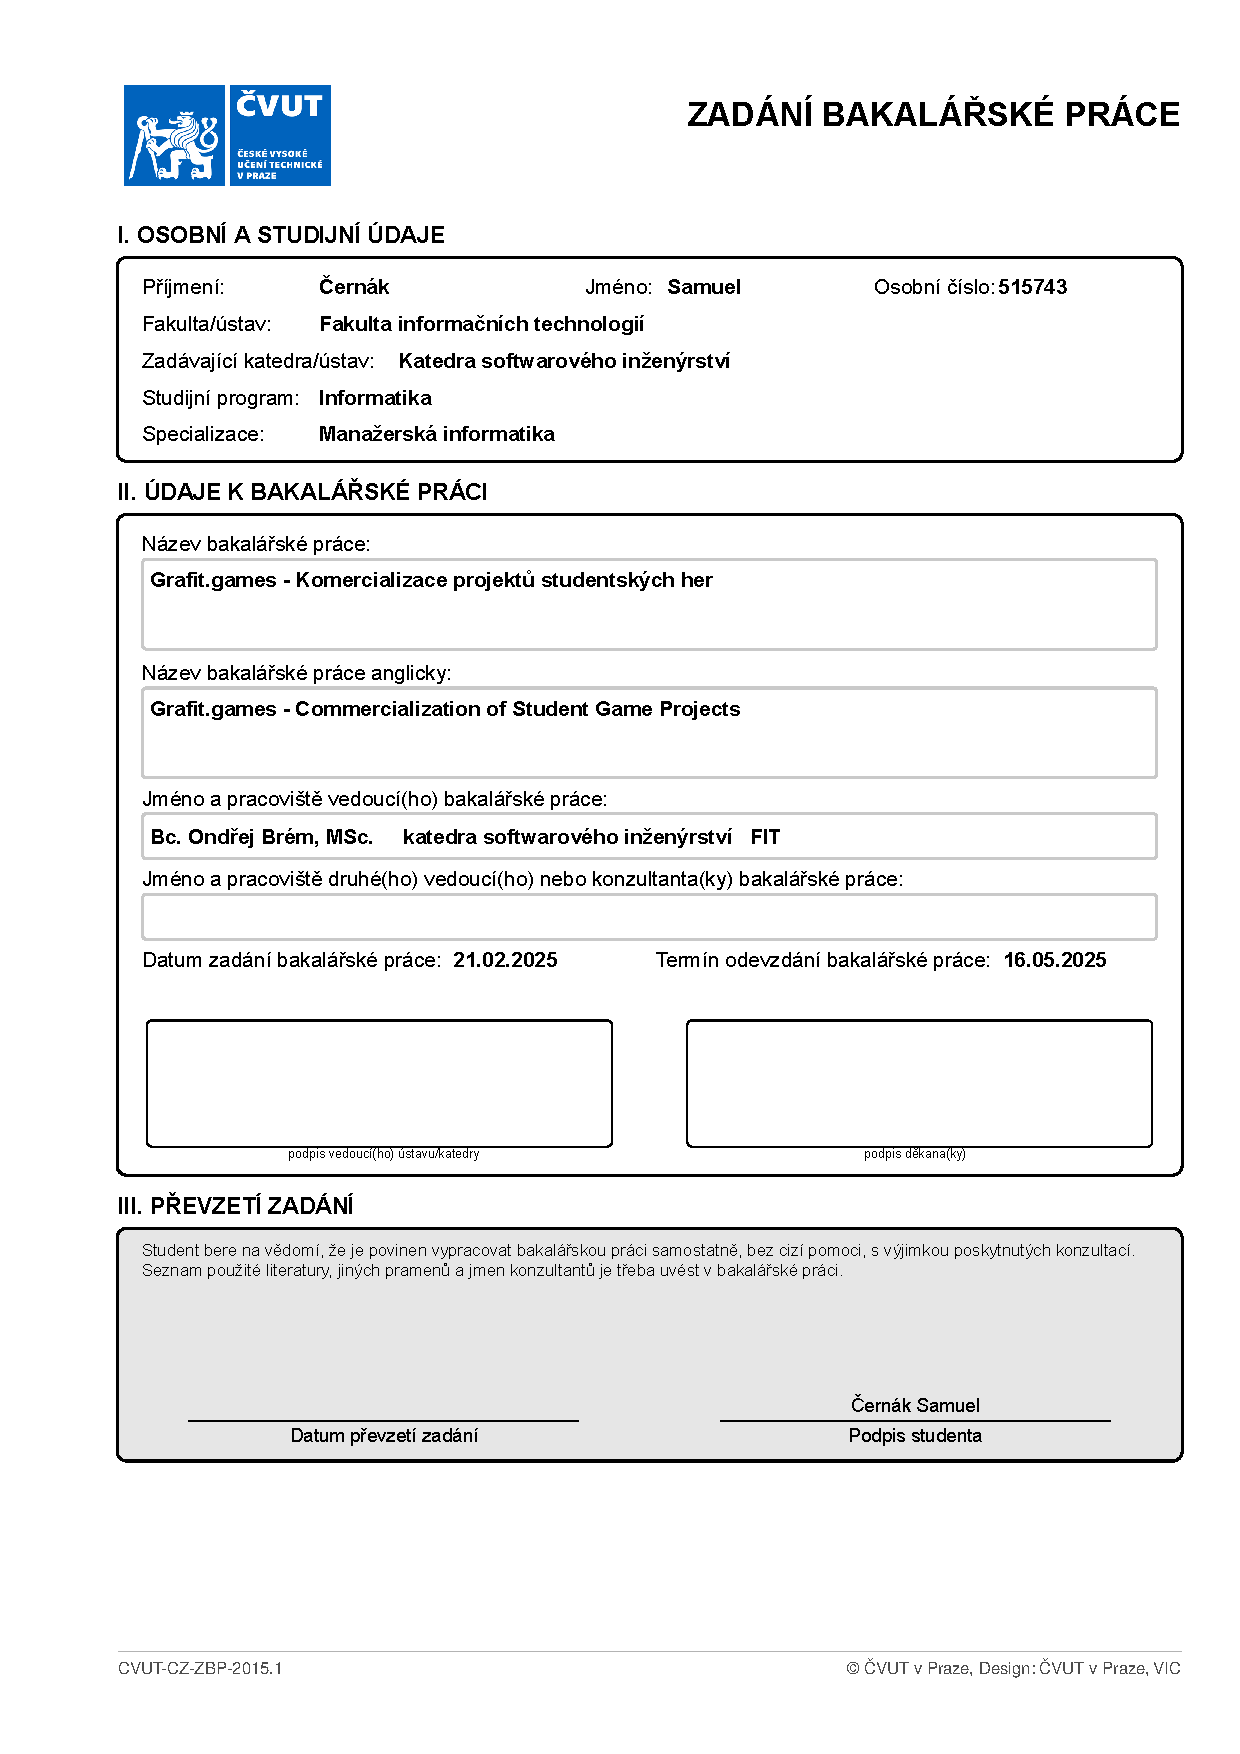
\includepdf[pages={1-}]{thesis-assignment.pdf} % replace this file with your thesis assignment generated from ProjectsFIT

\imprintpage % do not remove this command
\stopTOCentries
%%%%%%%%%%%%%%%%%%%%%%
% list of other contents END
%%%%%%%%%%%%%%%%%%%%%%

%%%%%%%%%%%%%%%%%%%
% ACKNOWLEDGMENT
% FILL IN / MODIFY
% This is a place to thank people for helping you. It is common to thank your supervisor.
%%%%%%%%%%%%%%%%%%%
\begin{acknowledgmentpage}
    I would like to express my sincere gratitude to Bc.~Ondřej Brém,~MSc., my thesis supervisor, for his dedication, guidance, feedback, and the considerable time and effort he devoted to this work. His expertise, patience, and willingness to discuss and challenge ideas were instrumental in shaping this thesis.
    I am also deeply thankful to Ing.~Jan~Matoušek, whose vision and support were invaluable in clarifying key decisions.
    Special thanks to Alica Seidlová for her editorial input, and to Nina Kubenová for helping me understand the~underlying regulation relevant to the project.
    I am grateful to Mgr. Dominik Vítek for his encouragement, and to Ing. Radek Richtr, Ph.D., for generously providing the website template and design language.
    Their support has been vital in bringing this thesis to~life.
\end{acknowledgmentpage} 
%%%%%%%%%%%%%%%%%%%
% ACKNOWLEDGMENT END
%%%%%%%%%%%%%%%%%%%


%%%%%%%%%%%%%%%%%%%
% DECLARATION
% FILL IN / MODIFY
%%%%%%%%%%%%%%%%%%%
% INSTRUCTIONS
% ENG: choose one of approved texts of the declaration. DO NOT CREATE YOUR OWN. Find the approved texts at https://courses.fit.cvut.cz/SFE/download/index.html#_documents (document Declaration for FT in English)
% CZE/SLO: Vyberte jedno z fakultou schvalenych prohlaseni. NEVKLADEJTE VLASTNI TEXT. Schvalena prohlaseni najdete zde: https://courses.fit.cvut.cz/SZZ/dokumenty/index.html#_dokumenty (prohlášení do ZP)
\begin{declarationpage}
I hereby declare that the presented thesis is my own work and that I have cited all sources of~information in accordance with the Guideline for adhering to ethical principles when elaborating an academic final thesis. 
In the course of~writing, I have used AI-assisted tools—such as language models—for support with stylistic editing, grammar refinement, and clarity improvements. All conceptual, analytical, and structural elements of the thesis remain my own.

I acknowledge that my thesis is subject to the rights and obligations stipulated by the Act No.~121/2000 Coll., the Copyright Act, as amended. In accordance with Section 2373(2) of Act No.~89/2012 Coll., the Civil Code, as amended, I hereby grant a non-exclusive authorization (licence) to utilize this thesis, including all computer programs that are part of it or attached to it and all documentation thereof (hereinafter collectively referred to as the "Work"), to~any and all persons who wish to~use the Work. Such persons are entitled to use the Work in any manner that does not diminish the value of the Work and for any purpose (including use for profit). This authorisation is unlimited in~time, territory and quantity.
\end{declarationpage}
%%%%%%%%%%%%%%%%%%%
% DECLARATION END
%%%%%%%%%%%%%%%%%%%%%%%%%%%%%%%%%%%%%%%%%%%%%%%%%%%%%%%%%%%%%%%%%%%%%%%

\printabstractpage % do not remove this command

%%%%%%%%%%%%%%%%%%%
% SUMMARY
% FILL IN / MODIFY
% OR REMOVE ENTIRELY (upon agreement with your supervisor)
% (appropriate to remove in most theses)
%%%%%%%%%%%%%%%%%%%
% \begin{summarypage}
%
%
% \end{summarypage}
%%%%%%%%%%%%%%%%%%%
% SUMMARY END
%%%%%%%%%%%%%%%%%%%

\tableofcontents % do not remove this command
%%%%%%%%%%%%%%%%%%%%%%
% list of other contents: figures, tables, code listings, algorithms, etc.
% add/remove commands accordingly
%%%%%%%%%%%%%%%%%%%%%%
% \listoffigures % list of figures
% \begingroup
% \let\clearpage\relax
% \listoftables % list of tables. Remove if you do not have any.
% \thectufitlistingscommand % list of code listings. Remove if you do not have any.
% \endgroup

%%%%%%%%%%%%%%%%%%%
% ABBREVIATIONS
% FILL IN / MODIFY
% OR REMOVE ENTIRELY
% List the abbreviations in lexicography order.
%%%%%%%%%%%%%%%%%%%
\chapter{\thectufitabbreviationlabel}
	
\begin{tabular}{rl}
a.s.    & Akciová společnost (Czech term for Joint-Stock Company)\\
CCPA    & California Consumer Privacy Act\\
CZK     & Czech Koruna (currency)\\
Dev     & Development\\
DLC     & Downloadable Content\\
ESRB    & Entertainment Software Rating Board (age rating)\\
EU      & European Union\\
EULA    & End-User License Agreement\\
FIT CTU & Faculty of Information Technology at the Czech Technical University\\
GDP     & Gross Domestic Product\\
GDPR    & General Data Protection Regulation\\
IP      & Intellectual Property\\
LLC     & Limited Liability Company\\
MVP     & Minimum Viable Product\\
OSVČ    & Osoba samostatně výdělečně činná (Czech for sole proprietorship)\\
PEGI    & Pan European Game Information (age rating)\\
PhD     & Doctor of Philosophy\\
QA      & Quality Assurance\\
R\&D    & Research and Development\\
s.r.o.  & Společnost s ručením omezeným (Czech term for LLC)\\
SWOT    & Strengths, Weaknesses, Opportunities, and Threats (analysis method)\\
UI      & User Interface\\
USA     & United States of America\\
UX      & User Experience\\
\end{tabular}
%%%%%%%%%%%%%%%%%%%
% ABBREVIATIONS END
%%%%%%%%%%%%%%%%%%%
\resumeTOCentries
\mainmatter\mainmatterinit % do not remove these two commands
%%%%%%%%%%%%%%%%%%%
% THE THESIS
% MODIFY ANYTHING BELOW THIS LINE
%%%%%%%%%%%%%%%%%%%

%---------------------------------------------------------------
% uncomment the following line to create an unnumbered chapter
% \chapter*{Introduction}\addcontentsline{toc}{chapter}{Introduction}\markboth{Introduction}{Introduction}
%%%%%%%%%%%%%%%%%%%%%%%%%%%%%%%%%%%%%%%%%%%%%%%%%%%%%%%%%%%%%%%%
%===============================================================
\chapter*{Introduction}\addcontentsline{toc}{chapter}{Introduction}\markboth{Introduction}{Introduction}
%===============================================================
Each year, students pour creativity, effort, and technical skill into developing original games as part of their studies. Yet once these projects are handed in and graded, they are often left unused---despite their potential to grow into successful products. This thesis explores why that happens and what can be done to change it.

Our focus is on student-created games at FIT CTU in Prague, Czechia. While the local environment shows promising signs---especially through strong private sector investment---many student projects fail to progress beyond the classroom. We believe this is largely due to a lack of entrepreneurial confidence and know-how among students, as well as the complexity and effort involved in commercializing a game. This thesis aims to investigate how a~simple, accessible support system could help bridge that gap.

This thesis examines the support currently available for game developers at~different stages of the creative process. Our goal is to consider the possible mechanisms for commercialization, evaluate and propose a system tailored to~our students’ needs. To validate our approach, we will conduct user sentiment testing and then describe a test run, including how we will evaluate its success or failure and plan subsequent steps. Ultimately, our broader objective is to improve entrepreneurial skills and mindset within the local community, and to inspire and motivate students to launch their own game ventures, equipping them with practical tools and confidence to navigate the industry.

Rather than going deep into the technical development of games, the selection and financing required to sustainably run an incubator, or creating a functioning university spin-out company, this thesis will instead focus on preparing the conceptual foundation for future implementation. Our goal is to design a~system---its processes, rules, and intended outcomes---to prepare the project for implementation. This approach allows us to test interest, gather feedback, and refine the model before any formal or financial commitments are made.

The thesis is divided into sections---each made up of several multiple chapters. The research part explores the game development process, academic entrepreneurship, and commercialization models---both locally at FIT CTU and internationally. In the design part we compare options and select a model suited for our needs. Then we move to practical steps: we prepare association rules, launch a recruitment website, collect interest and prepare a validation mechanism. The thesis concludes by reviewing the results, assessing whether the goals were met, and outlining future steps. We invite you to explore with~us how student creativity can be supported and transformed into real-world success.
%
%%%%%%%%%%%%%%%%%%%%%%%%%%%%%%%%%%%%%%%%%%%%%%%%%%%%%%%%%%%%%%%%
\clearpage % \clearpage if odd-numbered page ins't needed - otherwise \cleardoublepage
\setcounter{page}{1}
%
%===============================================================
\chapter{Academic Entrepreneurial Ventures}
%===============================================================

\begin{chapterabstract}
	Start-ups and spin-outs are powerful vehicles for transforming innovative ideas and research into market-ready products and services. In academia, these ventures not only drive technological and economic progress but also provide students with hands-on entrepreneurial experience and alternative career pathways. However, the process of launching and sustaining such ventures is shaped by national innovation ecosystems, regulatory environments, and varying institutional support systems. The chapter notes the differences between start-ups and spin-outs, explores the support structures available within universities, and highlights the practical and societal benefits of student involvement in these ventures. It also analyzes the challenges and opportunities faced by academic spin-outs in the Czech Republic’s innovation landscape and the game development sector.
\end{chapterabstract}

As universities continue to expand their role beyond traditional teaching and research, there is a growing emphasis on their capacity to drive innovation and contribute to local economic development. One of the broader aspirations of this work is to strengthen the local entrepreneurial ecosystem by empowering students to transform creative ideas into viable ventures. In this context, understanding the mechanisms behind start-ups, spin-outs and their potential benefits becomes essential.

%===============================================================
% \section{Start-Ups and Spin-Outs}
\textbf{Start-up} is a business newly established by an entrepreneur that aims to develop a unique product or service to meet market needs. Start-ups are characterized by innovation, high growth potential and often low revenue. They typically operate in uncertain environments, relying on venture capital\footnote{Capital can describe anything that has value - eg. machinery, intellectual property or financial assets.}, angel investors, or other funding sources to support their development.

\textbf{Spin-out} is a new company created from an existing organization, such as a university or a corporation, formed to commercialize developed research, intellectual property, or technology. Spin-outs benefit from the resources and expertise of their parent organizations while functioning as independent entities.

In academia, start-ups and spin-outs translate ideas and research into marketable products and services. Universities and research institutions support these ventures through incubators, technology transfer offices, and funding programmes. Academic spin-outs, in particular, utilize faculty expertise, patents, and support to drive innovation and economic impact.

%===============================================================
\section{The Impact of Academia-Driven Innovation}
Student spin-outs transfer theoretical early-stage research from universities to real-world applications. They are seen as an attractive alternative to patent licensing as they are more likely to impact the local economy. Spin-outs create jobs for highly skilled workers and provide valuable knowledge spillover for other companies.

Students taking part in spin-outs and start-ups can gain experience in entrepreneurship, practice business planning, market analysis, technology commercialization and more. Even unsuccessful undertakings provide valuable learning opportunities. Moreover, venturing offers an additional career path for students (particularly researchers facing limited job opportunities).

Academic ventures foster collaboration between students, faculty, and external actors such as industry partners. This strengthens the university's ecosystem for innovation and entrepreneurship. Successful undertakings improve the university's reputation and potentially attract more funding for research and other programmes.

Academic ventures have demonstrated the ability to adapt quickly to societal challenges. For example, during the COVID-19 pandemic, some quickly developed solutions to address urgent problems. Many also focus on solving pressing global problems, such as sustainability or healthcare challenges, contributing to broader societal benefits.

Commercial undertakings of students and academic staff offer many benefits, from driving local economic growth to fostering innovation and creating new career opportunities. Supporting these ventures is a logical step, as is encouraging the commercialization of student-developed games. Allowing finished games and projects to be forgotten is a wasted opportunity. By supporting these creations, universities can increase their impact, accelerate students' careers and strengthen the entrepreneurial ecosystem.

%===============================================================
\section{Academia-Driven Innovation in the Czech Republic and the World}
The commercialization and success rates of student ventures vary significantly across the world, reflecting differences in ecosystems, funding structures, and cultural attitudes toward entrepreneurship. It is useful to examine the state of innovation in the Czech Republic, to better understand the local potential for academic entrepreneurship.

In a study conducted by the Research, Development and Innovation Council in 2021, the Czech Republic demonstrated strong economic potential and a well-established industrial and research base. Investment in research and development reached a record CZK 121.9 billion (2\% of GDP). The country showed a high publication output, with over 80\% of research results published in indexed journals. Increasing international collaboration has driven excellence in specific scientific fields.

The study however concluded that challenges remain. The PhD completion rates are declining, reflecting low development of researchers' skills and professional capacities. Cooperation between the private and public sectors in research, development and innovation is limited. Innovation faces hurdles such as funding shortages and administrative burdens.

The Czech students perceive entrepreneurship as an attractive option for their future career paths. Addressing the systematic weaknesses while capitalising on the existing strengths can improve the Czech Republic’s competitiveness in research, development, and innovation on the global stage.

The gaming industry produces the Czech Republic’s most significant cultural export according to infiniteczechgames.com. Data by the Czech Game Developers Association from 2023 attributed the industry a turnover of CZK 7.52 billion with more than 98\% of it from abroad.

Mostly comprised of small studios, the industry employed over 2600 workers in 2023 - doubling since 2007. 71\% of those workers were under the age of 35 but only 48\% university-educated and only 21.4\% stated formal education as a source of their know-how. These numbers suggest that the field is vibrant and growing, but that the impact of universities and university-provided support is limited.

%===============================================================
\chapter{Game Development Processes}
%===============================================================

\begin{chapterabstract}
	The game development process is a series of interconnected stages taking creatives from an idea to a commercial product. Understanding of the~process allows a developer to make informed decisions, a supportive body to~provide targeted assistance and an investor to assess the state and outlook of a~project. The chapter breaks down each component of the process---from~planning, pre-production and production to testing, launch and post-launch activities. It especially focuses on the launch phase---requiring a~distinct set of competencies from marketing and distribution to niche legal and~financial expertise, often underrepresented in the technically and creatively oriented developer teams.
\end{chapterabstract}

Game development is not a single, linear task but a series of interconnected stages, each with its own distinct goals and requirements. A thorough understanding of the entire process is essential for any student team aiming to~successfully bring their game to the release stage---allowing them to anticipate challenges, allocate resources effectively, and make informed decisions at every step, from concept to completion.

%===============================================================
\section{Game Development Stages}
Game development is the process of designing, creating, and releasing video games. It includes writing, sound design, project management, programming and more. The process can be divided into distinct stages that focus on different aspects of the final product.
\cite{bramble_7-stages, rocket_6-stages}

%---------------------------------------------------------------
\paragraph{Planning Stage}
In the initial stage, game developers choose the genre that fits their vision the best, select viable art styles and gameplay mechanics, plan the game’s structure, content, and more. Changing, cutting or replacing later on can be straightforward in some aspects of the game and very challenging in others. Such aspects must be decided early on.
\cite{bramble_7-stages, rocket_6-stages}

%---------------------------------------------------------------
\paragraph{Pre-Production Stage}
The pre-production stage of game development requires artists, writers and designers to finalise important decisions. Feasibility, practicality and the worth of different design aspects is considered. Will the~game be fun to play and appealing to look at? Will it work properly, or~do some technical limitations need to be taken into account?
\cite{bramble_7-stages, rocket_6-stages}

%---------------------------------------------------------------
\paragraph{Production Stage}
After the decision-making, production of the game can start. It is at this stage when most of the code is written, levels are designed, game mechanics are tested, models, textures and visual elements start to appear.
\cite{bramble_7-stages, rocket_6-stages}

%---------------------------------------------------------------
\paragraph{Testing Stages}
Some form of internal testing is done throughout the entire process. Before the game is finalised however, developers tend to release test versions. This practice can be roughly divided into alpha and beta.

The \textit{alpha version} of the game already has the key mechanics and allows developers to assess playability. It might have placeholders for characters, surroundings or lack music. It is used for internal\footnote{refered to as closed} testing between staff members but can in some cases be available\footnote{refered to as open} to selected, passionate fans willing to help developers with playtesting.

The \textit{beta version} follows alpha. The game still requires a lot of work at this point but elements such as the environment and characters are approaching their final form. There still might be bugs present, glitches and exploits that need fixing, performance optimization required, and details missing. The game mechanics may still need to be balanced and server stability tested.\footnote{Betas can be open or closed too.}
\cite{bramble_7-stages, rocket_6-stages, esler_viable-games}

%---------------------------------------------------------------
\paragraph{Launch Stage}
During the launch stage the game is made available for the~public to play. This stage requires understanding the target market, audience, selecting a distribution channel, creating a strategy, and advertising. Additional support for players might be provided and feedback gathered.
\cite{bramble_7-stages, rocket_6-stages, esler_viable-games}

%---------------------------------------------------------------
\paragraph{Post-Launch Stage}
After the initial publication, developers might want to~release updates, patch bugs or even add new content, either as a free update or in the form of a purchasable extension. Continuation of a successful product allows it to extend its lifespan and provides a long-term fanbase.
\cite{bramble_7-stages, rocket_6-stages}

%===============================================================
\section{Launch Process in Detail}
While the students at the Faculty of Information Technology at the Czech Technical University (FIT CTU) often excel at designing and programming games, the launch phase is where many projects struggle. Unlike development, which follows a structured technical process, launching a game involves a complex and often unfamiliar set of tasks, from marketing and distribution to niche legal and financial specialties, budget planning, fundraising, assessing copyright protection, trademarks, creating contracts and more. A successful launch requires careful planning, strategic timing, and an understanding of~distribution platforms and promoting. Many of these steps are not immediately obvious but can determine whether a game finds an audience or gets lost in~an~oversaturated market.

%---------------------------------------------------------------
\subsection{Structural Requirements}
Ensuring a smooth and successful launch requires meeting critical structural requirements that impact a game’s performance, security, and compliance. Overlooking these factors can lead to negative user experiences, security vulnerabilities, and even regulatory consequences.

Before being released to the public, games need to be assessed and extensively tested to ensure stability and playability. The first thing a player interacts with is the UI---a launch screen or app---which therefore needs to be optimized. Settings such as the resolution, window size, language, subtitles, and~key bindings need to work properly. Accessibility and support options need to~be tested and credits/end game screens polished.\cite{silva_guide-to-release}

For games with online components, a reliable server infrastructure is crucial. Poor server performance can lead to lag or disconnects during traffic surges. Optimizing configuration, considering scalability and running stress tests before launch helps identify potential bottlenecks.\cite{sentika_how-to-optimize}

Major gaming platforms, from Steam to PlayStation, Xbox and mobile app~stores, have specific technical requirements. Failing to meet performance specifications or file size limitations can lead to rejection, or post-launch repercussions.\cite{apple-ios-apps}

Collecting and storing personal player data is best avoided in the case of small student-led projects. If collecting data is necessary, developers must comply with regional regulations such as the General Data Protection Regulation (GDPR)\cite{eu_gdpr} in Europe and the California Consumer Privacy Act (CCPA)\cite{doj_ccpa} in~the USA. These regulations require data to be anonymized, encrypted, safely stored and access to it minimized. Non-compliance can lead to severe penalties.\cite{silva_guide-to-release}

%---------------------------------------------------------------
\subsection{Operational Requirements}
A successful game launch relies on careful coordination of tasks and resources. While technical readiness is crucial, the operational aspects of the launch determine how smoothly the transition from development to release unfolds.

Best practices include creating a detailed timeline for launch-related activities and setting a realistic launch date. Mapping critical milestones helps teams avoid last-minute chaos.\cite{edgegap_pre-launch-list}

Effective launch coordination requires collaboration between developers, marketers, community managers, and support staff. Clearly defining individual responsibilities and establishing a contingency plan can help prevent miscommunication or overlooking tasks. A pre-launch meeting can align all team-members and prepare them for launch day chaos.\cite{palmer_planning-launch, edgegap_pre-launch-list}

Preparing announcements for player communication channels (e.g., Discord, Reddit) to address potential issues or provide updates can promptly address player inquiries and provide updates.\cite{palmer_planning-launch, edgegap_pre-launch-list}

%---------------------------------------------------------------
\subsection{Legal Requirements}
From a legal standpoint, publishing a game entails compliance with intellectual property laws, consumer rights regulations, and distribution agreements. Intellectual Property (IP) protection, including copy rights, trademarks, and patents, safeguards creators’ work. IP applies to a finished game, but might also restrict use of assets such as code, art, music, and branding.\cite{jd-supra_ip}

Ownership of IP varies depending on how a creation has been produced. If, for example, a developer creates a game independently, they generally retain full rights. In collaborative projects, or when work is commissioned, ownership can become complicated and must be defined in written contracts.\cite{silva_guide-to-release, jd-supra_ip}

When incorporating third-party source material such as characters, settings, or themes from movies, TV shows, or other media, licensing agreements must be secured. Even small references to copyrighted works can lead to legal action if not authorized.\cite{silva_guide-to-release, jd-supra_ip}

Beyond copyright, trademark protection can apply to titles, logos, and other branding elements. A trademark prevents competitors from using similar names or logos hence firstly ensuring that a game title and branding do not infringe on existing trademarks is crucial.\cite{dragon_copyright}

To legally include music in a game, two types of licenses can be obtained. A synchronization license grants the right to use the underlying composition whereas a master license grants the right to use a particular recording.\cite{iconcollective_music-license}

After the use of all assets has been approved an End-User License Agreement (EULA) needs to be drafted.\cite{silva_guide-to-release} It is used to set clear expectations and~legally protects the interests of both the game developer and the player. It ensures that the creator retains ownership of its software, provides a framework for~handling disagreements, limits the creator’s liability, and ensures compliance with data privacy laws (like GDPR and CCPA). The agreement also allows users to understand what they're legally allowed to do with the software and~provides specifications such as features and the functionality. Publishing platforms such as Steam provide a general EULA that usually covers the needs of a small game.\cite{docupilot_eula, steam_content-survey}

Developers must also ensure compliance with data privacy laws in the targeted market---the GDPR\cite{eu_gdpr} in Europe and the CCPA\cite{doj_ccpa} in the U.S. Data can generally only be collected if there is a lawful basis for it, a necessity for gameplay or user management and a clear explanation why and how it will be processed---usually in the EULA.\cite{dentons_eu-data-protection, gamota_data-privacy}

Traditionally, publishers required creators to obtain appropriate age ratings (e.g., PEGI, ESRB) based on the game’s content. On distribution platforms like Steam however, filling out a content survey suffices.\cite{steam_content-survey}

%---------------------------------------------------------------
\subsection{Marketing Requirements}
Marketing is the process of bringing a product to market. Successfully launching a game requires a strong marketing strategy to generate interest, attract customers, and maximize visibility.

During audience research, developers identify and attempt to understand the~target audience. Different genres appeal to different player demographics, and~marketing strategies should be tailored accordingly. Analyzing similar games, engaging with gaming communities or conducting surveys helps determine what resonates most.\cite{santos_pre-launch}

Creating a well-organized press kit is crucial for both media outreach and~promotions. It should include high-quality trailers, screenshots, game descriptions, developer quotes, and release details.\cite{impress_press-kit}

Building an online presence is a common strategy indie developers employ to~stand out, generate excitement and cultivate a dedicated community before launch. It is usually done through active participation---posting behind-the-scenes content, development updates, and engaging with fans---on social media platforms such as Reddit, Twitter, Instagram or TikTok. A website can serve as a central hub to direct an audience to. Its landing page should showcase press kit assets, include a newsletter signup option and other essential info.\cite{venkatesh_successful-release}

Influencer Partnerships---particularly with streamers and content creators aligned with the game’s genre---can significantly boost visibility.\cite{developer_introduction-to-marketing}

Finally, choosing the right distribution channel is key to a game’s launch and~long-term success. Different platforms cater to different audiences, offer unique visibility opportunities, and have varying revenue-sharing models. Developers must evaluate their goals and pick the best fit:
\begin{itemize}
	\item \href{https://store.steampowered.com/}{Steam}\footnote{accessible through https://store.steampowered.com/} is the largest digital distribution platform for PC games, accounting for 50-70\% of global PC game downloads.\cite{zuckerman_steam-statistics} It offers powerful tools for developers, including community forums, game analytics, and built-in marketing features such as Steam Wishlists. Listing a game on Steam involves submitting it through Steamworks, paying a \$100 fee (refundable after \$1000 in sales), and~adhering to the platform’s content guidelines. Steam has a fixed 30\% revenue split. The Steam Discovery Queue and algorithm-driven recommendations can boost sales provided the game gains enough initial traction through wishlists, reviews, and engagement.\cite{steam_wishlist,steam_partner-program,steam_discovery}
	\item \href{https://itch.io/}{Itch.io}\footnote{accessible through https://itch.io/} is a flexible, developer-friendly platform known for its supportive indie community and experimental games. Unlike Steam, Itch.io allows the developer full control over the revenue split, offering a pay-what-you-want pricing model. Itch.io however lacks the built-in discovery mechanisms and massive audience of Steam, requiring developers to rely on external marketing.\cite{carpenter_creator-day}
	\item \href{https://gamejolt.com/}{Game Jolt}\footnote{accessible through https://gamejolt.com/} emphasizes community-driven engagement with social-media-like features. Developers can post updates, interact with followers, and grow an~audience over time. Game Jolt offers flexible monetization options, such as one-time purchases, donations, or ad-supported releases. While good for building a player base, Game Jolt too lacks the commercial reach of Steam.\cite{game-jolt_help}
\end{itemize}

For many indie developers, the best approach is releasing on multiple platforms---launch a free demo on Itch.io or Game Jolt before transitioning to a release on~Steam.

%---------------------------------------------------------------
\subsection{Financial Requirements}
Understanding the financial requirements and strategies of game development determines the feasibility and success of a~project. From budget planning, securing initial funding to monetization strategies, developers must navigate several financial challenges.

% - - - - - - - - - - - - - - - -
\paragraph{Budget-Planning} A well-structured budget---commonly created through a~task breakdown\cite{linkedin_budget}---allocates funds across three primary areas:
\begin{itemize}
	\item \textbf{Development} includes salaries, outsourcing (e.g., music, voice acting), and~tools (software/hardware).\cite{eduonix_costs}
	\item \textbf{Marketing} covers promotional campaigns, ads, influencer partnerships, and~events.\cite{eduonix_costs}
	\item \textbf{Post-Launch Support} includes updates, fixes, server maintenance, and customer support.\cite{eduonix_costs}
\end{itemize}

% - - - - - - - - - - - - - - - -
\paragraph{Monetization Strategy} Choosing the right monetization strategy ensures sustainable business operations, allows investment into high-quality contributors and assets and incentivises innovation:
\begin{itemize}
	\item \textbf{Freemium} offers free access to the base game with revenue generated through ads or in-app purchases (e.g., skins).\cite{hubka_game-monetization}
	\item \textbf{Premium} involves an upfront fee for the game and is sometimes supplemented by paid expansions.\cite{hubka_game-monetization}
	\item \textbf{Subscription} provides access to the product throughout recurring payments (less common for indie games).\cite{hubka_game-monetization}
\end{itemize}

% - - - - - - - - - - - - - - - - 
\paragraph{Fundraising} Larger projects often require funding, which may come from several sources:
\begin{itemize}
	\item \textbf{Self-Funding} is commonly used by indie game developers until external funding is secured.\cite{perforce-stoftware_tips}
	\item \textbf{Publishers} traditionally provide financial support and marketing expertise but may require revenue-sharing agreements.\cite{perforce-stoftware_tips}
	\item \textbf{External investors} can financially back a project in exchange for equity, or~profit-sharing.\cite{perforce-stoftware_tips}
	\item \textbf{Crowdfunding platforms} such as \href{https://gamefound.com/en}{Gamefound}\footnote{accessible through https://gamefound.com/en} or \href{https://www.kickstarter.com/}{Kickstarter}\footnote{accessible through https://www.kickstarter.com/} allow developers to raise funds directly from potential players but rely on strong promotional efforts.\cite{perforce-stoftware_tips}
	\item \textbf{Organizations} in the gaming (eg. Unreal Engine) or education space may offer competitive grants to support prospective indie developers.\cite{perforce-stoftware_tips, unreal-engine_grants}
\end{itemize}

Lastly, when monetizing a game, the benefits of operating as a company should be considered. Starting a company is not strictly required and might entail upfront fees but provides legal protection, simplifies tax compliance, and can improve credibility when negotiating contracts with investors or publishers.\cite{expats_company-or-individual}
%===============================================================
\chapter{Our Games and Commercialization Support Options}
%===============================================================

\begin{chapterabstract}	
    FIT CTU offers a robust Informatics program with a specialization in computer graphics, combining theoretical foundations with hands-on coursework in areas such as programming, visualization, and user interface design. The faculty regularly organizes events like GameJams and supports a range of student-driven game projects, resulting in a diverse portfolio of innovative games. While students benefit from university-wide initiatives, incubators, and career development programs that help translate creative projects into viable ventures, entrepreneurial support is not directly embedded within FIT CTU and no options are specialized for game developers. The chapter details the game development education available at FIT CTU, showcases notable student projects, and outlines the ecosystem of events and support services that nurture both technical and entrepreneurial skills.
\end{chapterabstract}

Game development is an integral part of FIT CTU’s academic and extracurricular offerings. The Informatics programme, with its computer graphics specialization, provides students with a thorough foundation in both the theory and practice of game creation. As part of our effort to strengthen the support provided and improve the local entrepreneurial ecosystem, it is essential to understand the current opportunities available for creative development and commercialization within FIT CTU.

%===============================================================
\section{Game Development at FIT CTU}
The Faculty of Information Technology at the Czech Technical University (FIT CTU) offers a range of courses and events dedicated to game development. Currently, the faculty offers a single study programme - Informatics - which includes several specializations. Of particular relevance is the computer graphics specialization, which combines theoretical foundations with practical experience. Core theoretical courses include Computer Graphics Programming, Modern Visualisation Technologies, and Machine Vision and Image Processing, while more hands-on experience is provided through courses such as Multimedia and Graphics Applications, Programming of Graphic Applications, and User Interface Design.

In addition, FIT CTU is preparing a new study programme - Applied Informatics - which will introduce three new specializations: Game Development, Graphics, and Computer Vision. This programme is expected to offer a stronger emphasis on practical experience and expand the number of study places available in game-related fields. As a result, a broader range of student-developed games is anticipated - many of which could benefit from structured entrepreneurial support.

Game development is also integrated into other CTU courses, such as Team Software Project, where students have the option to work on game-rated projects as part of their coursework.

The FIT CTU GameJam is another key event fostering game development. Held over an extended weekend, this 48-hour challenge tasks students with creating a computer game from scratch. Participants work either individually or in teams, and receive guidance from experienced industry professionals. The event cultivates teamwork, creativity, and showcases students’ technical and artistic talents.

Overall, multiple study paths at FIT CTU support the creation of original games - whether through specialized coursework, faculty-led research, extracurricular events, or student-driven initiatives. The faculty provides an environment in which aspiring developers can hone their skills and bring their ideas to life.

%===============================================================
\section{Example Games from FIT CTU}
Over the years, students at the FIT CTU have created a wide range of original, comical and technically impressive games. These projects often combine creative storytelling and original game mechanics and are developed as part of coursework, bachelor’s or master’s theses, Game Jams or independent student initiatives.

\begin{figure}[H]
    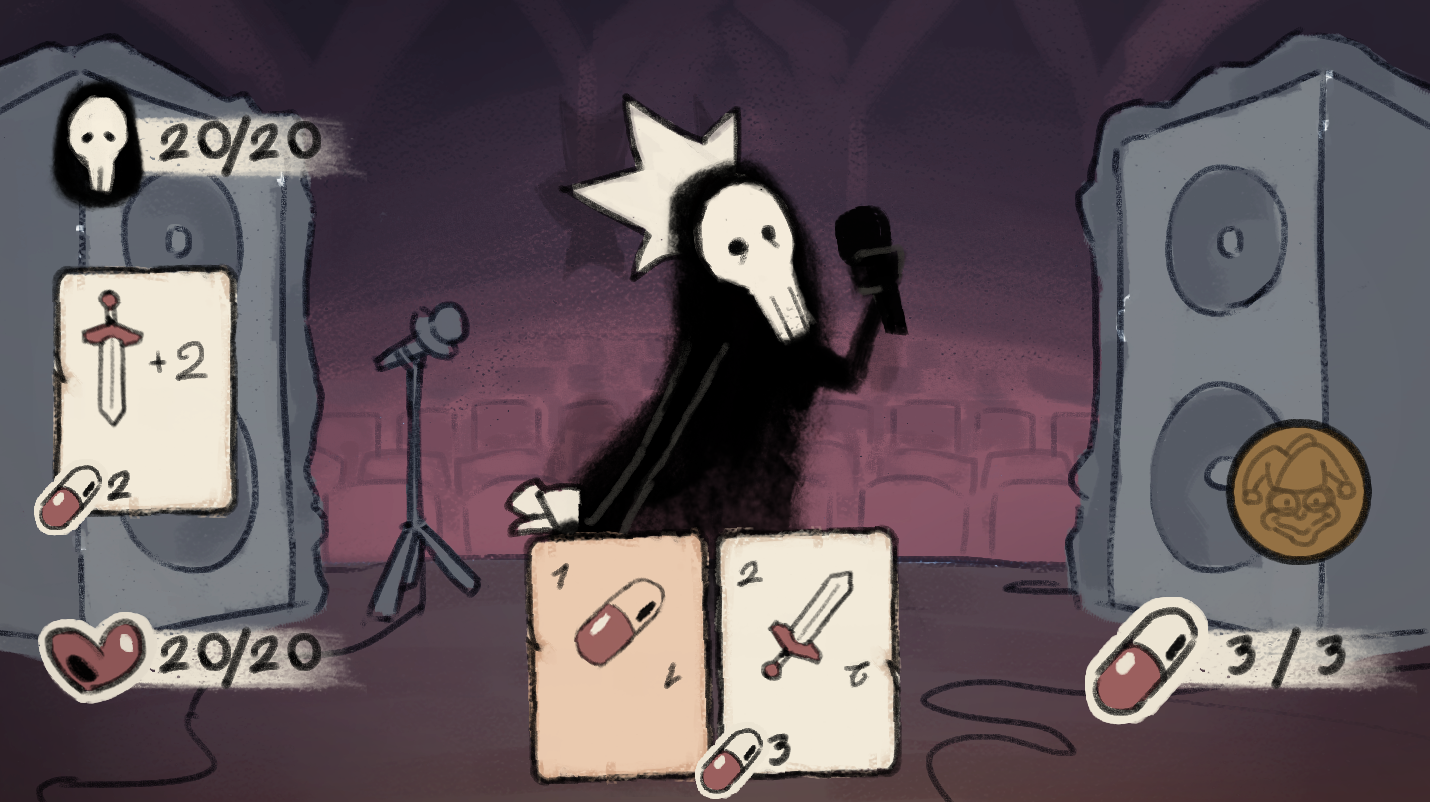
\includegraphics[width=0.9\textwidth]{encore.png}
    \caption{Image from the GameJam's Itch.io~[citation]}
    \label{fig:encore-picture}
    Encore! developed during the 2024 GameJam by Belonzik and TheMultiplexx is a dueling card game with outstanding attention to detail, exploring the theme of death. It stands out for its excellent graphics, well-crafted audio, immersive story, and even professional-grade narration.
\end{figure}

\begin{figure}[H]
    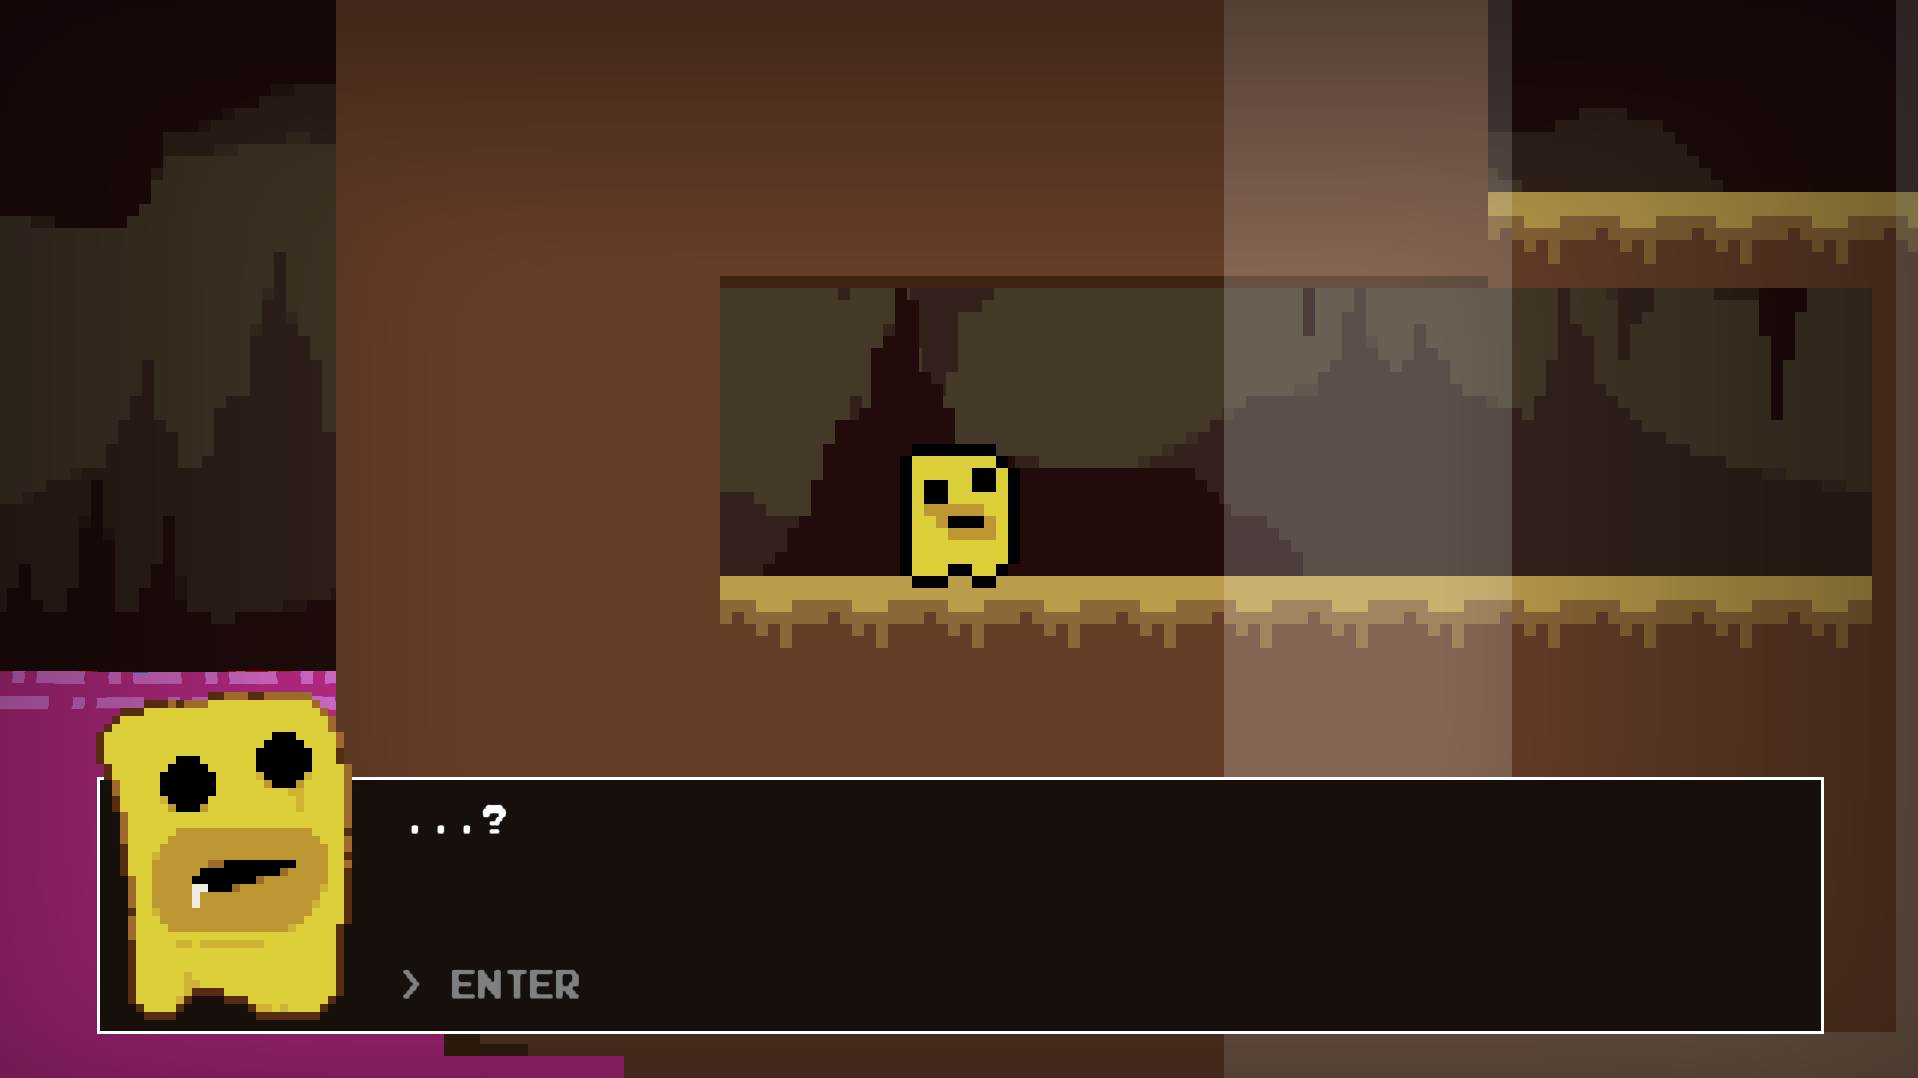
\includegraphics[width=0.9\textwidth]{liminal.png}
    \caption{Image from the GameJam's Itch.io~[citation]}
    \label{fig:liminal-picture}
    Liminal! by HyperCubic Studio was developed during the 2024 GameJam too. This short platform puzzle game traps the player in a twisted TV show. The game’s colourful visuals are beautiful, cohesive and extensively polished. It boasts original mechanics and is full of details in the sounds, menu items and dialogue.
\end{figure}

\begin{figure}[H]
    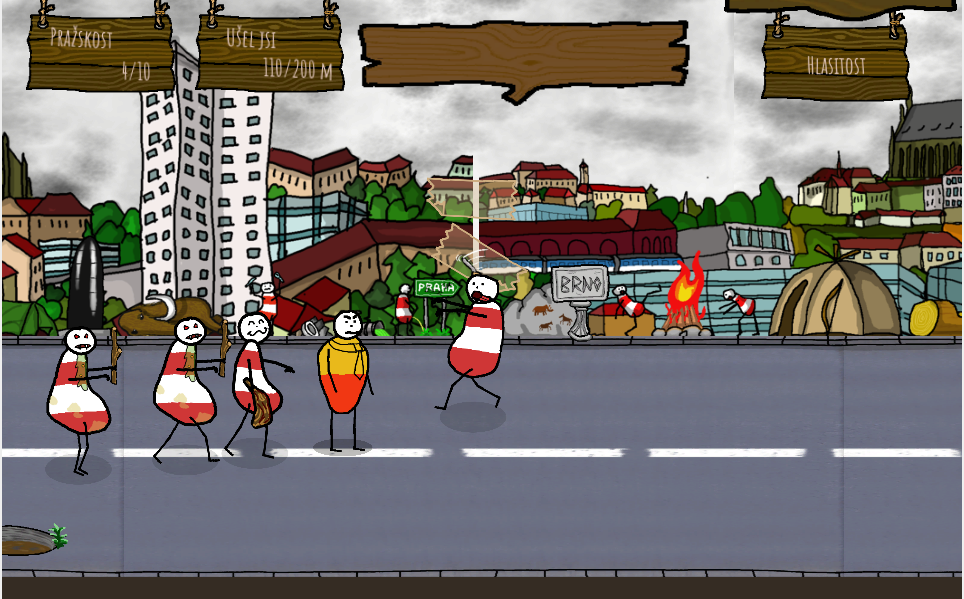
\includegraphics[width=0.9\textwidth]{brno.png}
    \caption{Image from the GameJam's Itch.io~[citation]}
    \label{fig:brno-picture}
    Escape from Brno was created during the 2022 GameJam by Trampod, SharpFoxDev, benjaminhejl, leia12321 and VAHAnima. This side-scrolling dodger won the popular vote among the participants. Its humorous sound design, cohesive graphics, and intuitive gameplay make it feel natural and engaging.
\end{figure}

\begin{figure}[H]
    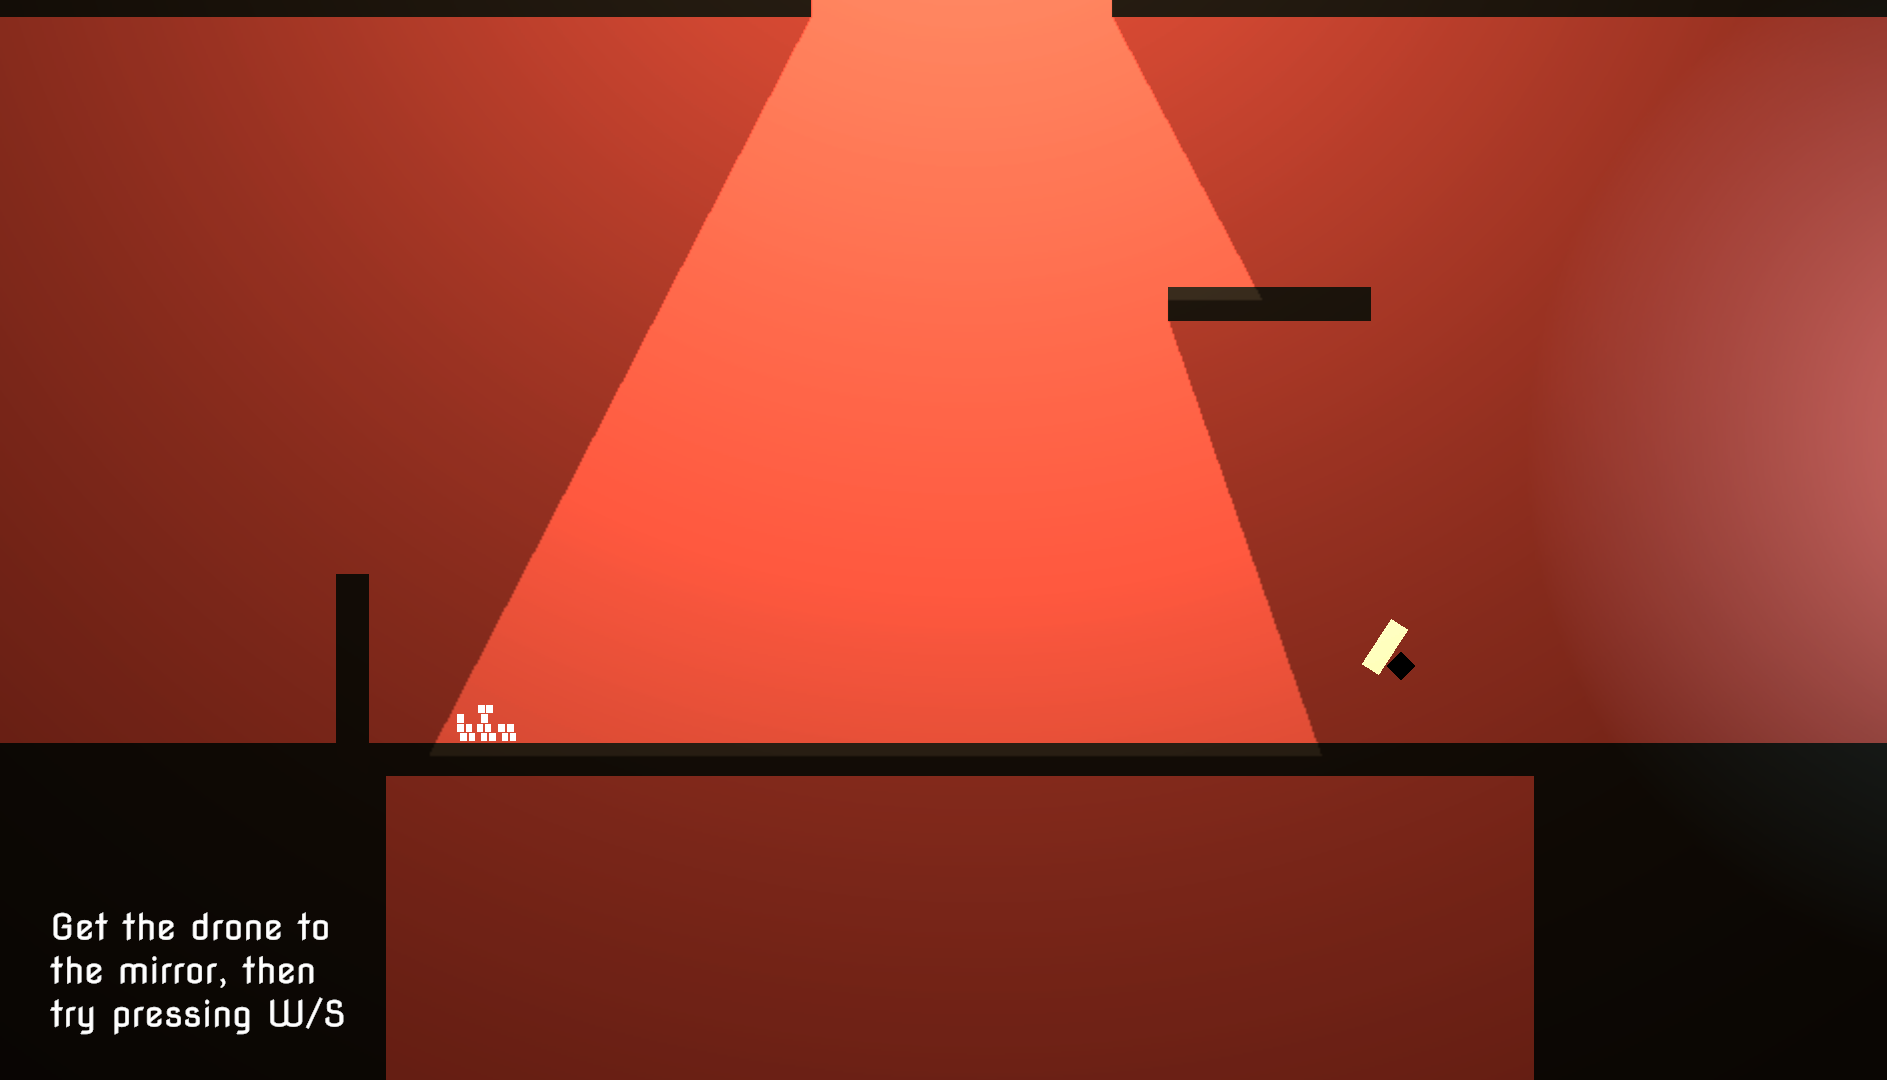
\includegraphics[width=0.9\textwidth]{subject.png}
    \caption{Image from the GameJam's Itch.io~[citation]}
    \label{fig:subject-picture}
    Subject 42 was created by LukyDrum during the 2023 GameHack. This game puts the player in control of a robot’s AI as they solve puzzles and navigate three intriguing levels. A fitting sound-track and a voice sarcastically commenting on the player’s performance contribute to its unique style and storytelling.
\end{figure}

%===============================================================
\section{Local Student Entrepreneurship Support}
While FIT CTU does not currently provide entrepreneurial support, it does facilitate cooperation with industry partners and manages grants for research labs. The university takes over the responsibility of arranging access to dedicated incubators and coaching centers. These initiatives help students refine their business ideas and develop their skills.

One such initiative is InQbay, a CTU-wide programme supporting student, phd, and faculty entrepreneurs. It offers individual coaching, workshops, tutorials, networking events, and access to legal, tax, and marketing consultants.

In addition, the CTU career centre offers an eight-week long entrepreneurship course. It covers ideation, market research, business plan creating, pitching a project, gathering feedback and seeking mentors or investors.

%===============================================================
\chapter{University-Based Programmes Facilitating Entrepreneurship}\label{chap:incubators}
%===============================================================

\begin{chapterabstract}
    University incubators have become essential engines of innovation, offering mentorship, funding, workspace, and industry connections to early-stage start-ups. They bridge academia and industry, helping students and researchers overcome barriers to commercialisation. Specialised game incubators have recently emerged to address the unique needs of game development teams. This chapter surveys prominent incubator models and their offerings in the Czech Republic and internationally. The analysis covers how the programmes are structured, select participants, and propone collaboration, as well as the challenges and best practices in supporting student ventures from ideation through launch.
\end{chapterabstract}

Game development ventures face unique challenges---such as rapid product cycles and fierce market competition---making commitment to a commercial project difficult. Tailored initiatives---providing targeted mentorship, initial capital, and industry connections---can help teams accelerate the journey from prototype to market-ready product and lower the barriers to entry for aspiring founders, highlighting the need for their thoughtful understanding.

\textbf{Start-up incubators} help develop and refine high-potential business ideas. They usually operate locally and provide resources over a span of one to five years. Incubators tend to offer product development guidance, on-demand co-working space, legal consultation, networking opportunities and mentorship.
\cite{harward-incub-accelerator}

\textbf{Start-up accelerators} are short, intensive programmes for early- or mid-stage founders. Accelerators are more structured than incubators and outline specific steps to create a scalable business. They often have an alumni and investor network and offer funding in return for stake in the company. Participants usually go through intensive mentorship from industry leaders on fundraising, product development, and growth marketing.
\cite{harward-incub-accelerator}

Both start-up incubators and accelerators are typically selective in who they allow into their programme. Whilst incubators provide the learning environment and physical resources to help an idea succeed, accelerators compress years worth of learning and growth into the span of a few months.
\cite{harward-incub-accelerator}

%===============================================================
\section{Prominent Traditional Incubator Functions}
Major university-based incubators offer a variety of functions and services. Primarily, they provide some kind of mentorship---from industry experts, successful entrepreneurs, and or alumni. They run workshops or tutorials to help develop entrepreneurial skills and other relevant competencies. For example The Macquarie University (in Sydney) Incubator’s mentor programme directly matches founders with experts to help them navigate the journey and share their insights.
\cite{Bonenkamp_incubators, Macquarie-incubation}

Incubators also tend to provide free or subsidized facilities. RWTH Innovation grants access to research facilities. Lund University’s VentureLab even offers free office space, coffee and fruit.
\cite{rth-innovation, lund-incubator}

Many incubation programmes provide direct capital\footnote{Capital can describe anything that has value - e.g., machinery, intellectual property, or financial assets.}, or help start-ups secure grants and investments. The UnternehmerTUM offers €5~000 for prototyping in their incubator, a €25~000 project budget in their accelerator and up to €250~000 in total funding. Cambridge Enterprise invested £6.47 million in 37 spinout companies (from 2023 to 2024). SETsquared helped raise £5~billion in investments.
\cite{unternehmertum, cambridge-venture, setsquared}

Incubators typically facilitate connections with investors, corporate partners, and other starting ventures. For example, over 6 500 companies have participated in the SETsquared programmes and Startup Autobahn partners with companies like Porsche and Daimler.
\cite{setsquared, autobahn}

Some incubators specialise in specific industries or technologies, support sustainability and social impact. Polihub focuses on deep tech start-ups, Wyss Zurich emphasizes regenerative medicine and robotics and Tartu University CDL-Estonia specialises in digital government and cybersecurity. EIT Climate-KIC supports climate-related start-ups.
\cite{polihub, wyss-zurich, estonia-creative-destruction, climate-strategy}

Moreover, incubators promote global competitions and highlight successful alumni as role models for incoming students and upcoming entrepreneurs. Cambridge Enterprise supported Raspberry Pi and the alumni of Yes!Delft include Ampelmann, a maritime tech company. EUT+ Incubation Program’s participants get to compete in the EUt+ Finals against the best teams from EUt+ campuses.
\cite{cambridge-raspberry, yes-delft, cuni-nic}
%===============================================================
\section{Prominent Game Incubators}
Game-focused incubators are beginning to emerge worldwide, aiming to nurture students and graduate creations into successful ventures. 

Gamebaze is an incubator formed by a joint initiative (between Game Cluster, JIC/KUMST and the GameDev Area) in Brno. It supports gaming-related start-up projects and is part of Czechia's robust gaming education ecosystem. It also facilitates partnerships with local studios like Warhorse Studio.
\cite{infinite-uni}

Sweden Game Arena---located in Skövde---unites a game development bachelor's and master's programme with a successful incubator under one umbrella. This ecosystem supports students by offering practical collaboration opportunities with a large number of game companies and access to industry events such as the Sweden Game Conference.
\cite{game-arena, education-msc-game-dev}

Game Hub Denmark operates in three cities---Grenaa, Aalborg, and Viborg. It includes facilities like the BizHub for secondary school students, Aalborg University Game Hub for entrepreneurs, and Roof Creative Industries Incubator in Viborg---part of one of the best animation schools in the world. The initiative also collaborates internationally---in typically EU-funded development projects---to expand opportunities for game start-ups.
\cite{gh-denmark}

When it comes to financing, The NYU Game Center Incubator grants its participants \$15~000 per team. The programme begins with in-person workshops and coworking sessions, transitioning to remote collaboration for a remainder of the year. The mentors include producers and industry professionals and the incubator partners with major industry players like Sony and Microsoft.
\cite{nyu-game-center}

GameBCN in Barcelona, Spain is a 5 months long programme accommodating teams from all over the world. It includes 90 hours of training---on production, marketing, and business---and feedback from industry professionals on monthly meetings. The selected companies are not required to give up equity.
\cite{strategy-incubation}

On the other hand, Carbon Incubator from Bucharest, Romania---catering primarily to indie developers from Eastern Europe---requires their incubated companies to give up 10\% of revenue. The share rises to 20\% in their acceleration programme and to 30\% for companies receiving funding.
\cite{strategy-incubation}

%===============================================================
\section{Entrepreneurship Support at FIT}
While FIT CTU does not currently provide entrepreneurial support, it does facilitate cooperation with industry partners and manages grants for research labs. The university takes over the responsibility of arranging access to dedicated incubators and coaching centres. These initiatives help students refine their business ideas and develop their skills.
\cite{fit-rozvoj}

One such initiative is InQbay, a CTU-wide programme supporting student, phd, and faculty entrepreneurs. It offers individual coaching, workshops, tutorials, networking events, and access to legal, tax, and marketing consultants.
\cite{inqbay}

In addition, the CTU career centre offers an eight-week long entrepreneurship course. It covers ideation, market research, business plan creating, pitching a project, gathering feedback and seeking mentors or investors.
\cite{kc_podnikni-to}
%===============================================================
\chapter{Student Venture Support Options}
%===============================================================

\begin{chapterabstract}
    While student game developers often excel at the creative and technical aspects of game creation, the transition from prototype to commercial product presents a host of new challenges - including legal and financial complexities. This chapter explores legal and organizational partnership formats for supporting student ventures, highlighting the limitations and emerging best practices.
\end{chapterabstract}

University incubators play a critical role in fostering student-led innovation - particularly in game development, where access to funding, mentorship, and infrastructure can make or break a start-up. Most university incubator programmes operate under the non-profit umbrella of their institutions. While this structure limits their ability to generate profit, it enables them to offer services such as mentoring, business guidance, co-working space, and financial assistance - often at no cost to students. Their primary goal is not immediate profit but rather fostering entrepreneurship and innovation.

Although some university incubators seek returns through royalties, equity ownership, or repayable loans, even large institutions often struggle to achieve financial self-sufficiency. As a result, these programmes are typically supported through a mix of institutional funding, public grants, corporate sponsorship, and alumni donations.

In many cases, incubators also manage the licensing of intellectual property created on university premises, including student projects - especially when the university retains certain rights, as is the case at FIT CTU. 

Commercializing student-developed games introduces legal and organizational complexities. Students must select suitable business structures and comply with tax and labor regulations. Incubators can simplify this process by incorporating ventures - protecting students from personal liability, facilitating profit-sharing and fair ownership.

%---------------------------------------------------------------
\section{Student Partnership Formats}
University incubators in the Czech Republic can support students in various ways, each offering unique advantages and constraints.

% - - - - - - - - - - - - -
\subsection{Supporting a Student-Led Venture}
\label{sec:label-supporting-student-venture}
One common method for universities to support student-led ventures is through structured partnerships, which allow students to operate independently while receiving institutional support. Common Legal Structures for Student Ventures include:
\begin{itemize}
    \item \textbf{Sole Proprietorship (OSVČ)} - ideal for ventures conducted individually. Requires no initial capital, can be registered by filing a unified registration form and paying an administration fee of CZK~1~000. The downside is full personal liability for any incurred debts and losses.
    \item \textbf{Limited Liability Company (s.r.o.)} - commonly used by small teams. Offers liability protection but requires structured book-keeping. Can be created with an initial capital of CZK~1 by concluding a memorandum of association (notary approval usually costs under CZK~10~000) and listing in the commercial register (administrative fees arround CZK~2~700 when done by a notary). 
    \item \textbf{Other - Joint-Stock Company (a.s.)} or Limited Partnership (komanditní společnost) may be appropriate for large projects seeking investment. Setting them up and adhering to the tax code is complex.
\end{itemize}

University incubators can support student-led venture through several financial mechanism:
\begin{itemize}
    \item \textbf{Loans} - repayable financing provided with agreed-upon terms and interest rates.
    \item \textbf{Equity Investment} - capital exchanged for partial ownership. Some non-profit structures cannot hold equity or engage in unlimited liability partnerships and need to have their business activity aligned with their defined purpose.
    \item \textbf{Grants} - non-repayable funding, often provided by non-profits. Can offer tax benefits to supporting organizations.
\end{itemize}

% - - - - - - - - - - - - -
\subsection{Employing Students}
University incubators could employ students directly or through subsidiary game development firms and compensate them for their contributions:
\begin{itemize}
    \item \textbf{Standard employment contracts} - developers receive a stable salary. Employers generally contribute 33.8\% (2.1\% towards sickness insurance, 21.5\% towards pension insurance, 1.2\% towards state employment policy and 9\% towards health insurance) while employees contribute an additional 6.5\% to social-security, 4.5\% towards health insurance and 15\% income tax. 
    \item \textbf{Freelance/contractor agreements}  - students work as independent contractors. They are required to register as sole proprietors, pay a 15\% income tax, and after deducting expenses pay 29.2\% social-security (if their yearly profits exceed CZK~111~736) and 13.5\% health insurance.
    \item \textbf{Internship programmes} - often tied to academic curriculum and enabled by scholarships funded by universities or industry partners. They must comply with Czech labor laws.
\end{itemize}

% - - - - - - - - - - - - -
\subsection{Allowing a Form of Ownership in the Incubator}
Students might also be allowed to hold equity in the incubator or its affiliated entities. This approach can minimize tax-burden and incentivize effort. Formats include:
\begin{itemize}
    \item \textbf{Paying out dividends} - distribution of profits to student shareholders. Such an approach requires the correct legal structure (in the Czech Republic usually an a.s., but can also be done through an s.r.o.) and has to be contractually defined. Transferring shares involves a CZK~2~000 administrative fee. Corporate profits are taxed 21\% and dividends an additional 15\%.
    \item \textbf{Profit distribution} - a cooperative (družstvo in the Czech Republic) allows members to participate in governance and share profits. At least 10\% of profits must be retained in a fund, with the rest distributed (subject to 21\% corporate and 15\% income tax). Initial costs include around CZK~3~000 for drafting statutes, CZK~10~000 for notarial certification and CZK~2~700 for listing in the commercial register.
\end{itemize}

%---------------------------------------------------------------
\section{University Incubator Legal Structure}
University incubators in the Czech Republic can take on various legal structures, each offering unique advantages and constraints.

% - - - - - - - - - - - - -
\subsection{Non-Profit Integration}
Many university incubators are structured as non-profit entities and integrated into the University's body. They are allowed to receive funding from public and private sources but focus on student development rather than profit-making. Common non-profit structures include:
\begin{itemize}
    \item \textbf{Student Clubs or Organizations} - informal collectives within universities usually offering peer-to-peer support and networking. Operations must strictly adhere to university policies and governance.
    \item \textbf{Joint Ventures with Private Companies} - often referred to as Public-Private Partnerships are not a legally described structure in the Czech Republic. Universities may partner with established game studios or tech firms to provide the required services.
    \item \textbf{Non-Profit Organizations} -  more formalized structures capable of applying for public grants and private donations. They are not allowed to be run for the sole purpose of generating profit.
    \begin{itemize}
        \item \textbf{Foundations (nadace)} - manage assets (exempt from tax) for charitable, religious, or public benefit goals. They are established by a notarial deed with an initial endowment (no minimal amount is specified) and by being listed in the foundations register. Endowments are protected and only earnings generated by its activities are expended. Foundation disclose annual financial reports, undergo audits and are restricted from participating in unlimited liability partnerships.
        \item \textbf{Funds (nadační fondy)} - provide access to the entire endowment. They focus on fundraising for specific causes or a time-bound project. Funds are registered by a notarial deed and by formulating governing statutes. They require no minimum capital, undergo lighter oversight but still disclose their activities.
        \item \textbf{Registered Institutes (ústavy)} - conduct educational, scientific, or cultural activities. They are established by concluding a memorandum of association, registering in the commercial register and have to undergo annual audits if revenues exceed CZK~40~million. Entrepreneurial activities must be supportive in pursuing the institute’s purpose.
    \end{itemize}
\end{itemize}

% - - - - - - - - - - - - -
\subsection{University-Owned Spin-Off Company}
Some universities establish separate, fully or partially owned entities. These must distribute gains to maintain the university’s nonprofit status. Common formats include:
\begin{itemize}
    \item \textbf{S.R.O. (Limited Liability Company)} - a university-owned company that partners with student teams created following the points mentioned in [chapter before].
    \item \textbf{A.S. (Joint-Stock Company)} - suitable for large ventures seeking external investment, requires initial capital of at least 2 million CZK.
    \item \textbf{Cooperative Structure }- a collective ownership model where students, faculty, and external partners share decision-making and profits. A cooperative (družstvo in the Czech Republic) is a corporate entity requiring a minimum of 3 members. It is founded by concluding a memorandum of association (notary approval usually costs under CZK 10000) and by listing the company in the commercial register (notary fee usually around CZK 2700). Profit distribution rules need to be outlined in the cooperative’s memorandum and can include criteria beyond capital contributions  - such as the performance of specific segments of the organization. Distributed profits are subject to a 21% corporate tax and a 15% personal income tax.
\end{itemize}


\externaldocument[nocite]{build/text/chapters/gave-dev}[url=text/chapters/game-dev]
\externaldocument[nocite]{build/text/chapters/support-formats}[url=text/chapters/support-formats]
\externaldocument[nocite]{build/text/chapters/launch-&-testing}[url=text/chapters/launch-&-testing]
\externaldocument[nocite]{build/text/chapters/programme}[url=text/chapters/programme]
\externaldocument[nocite]{build/text/appendix}[url=text/appendix]
%===============================================================
\chapter{Legal Structure for Our Programme}\label{chap:legal}
%===============================================================

\begin{chapterabstract}	
    Student-led game development is inherently creative and unpredictable, often lacking the business structure needed to succeed in a competitive market. Grafit.games can provide that structure. This chapter evaluates various legal models for university-affiliated incubators, ultimately proposing a phased approach beginning with informal student clubs and transitioning into a cooperative. The cooperative model has been chosen for its democratic governance, shared ownership, ability to fairly distribute profits among members, and low bureaucracy. It incorporates informal teams, providing a legal shell. The chapter provides statutes—describing membership, governance, and capital contributions---and guides creation of the entity. Additionally it describes the handling of Intellectual property rights using non-exclusive licences---allowing the incubator to commercialise games and student developers to retain rights to their work.
\end{chapterabstract}

Transitioning a prototype to a market-ready product is an exciting yet formidable journey. Providing mentorship and consulting goes a long way in facilitating that mission. Game development ventures—particularly at the student level—are unpredictable by nature---they rely on creative momentum in a competitive market. As such, navigating the legal, financial, and administrative landscape can pose an insurmountable obstacle. In section \ref{sec:swot}, it led to the conclusion that business support should be a prominent feature of the programme. While such services can begin informally, with growing complexity establishing a formal legal structure becomes necessary. Facilitating consistency, effective management of responsibilities, and ensuring long-term sustainability, the selection of an appropriate legal structure is critical.

%===============================================================
\section{Selecting a Legal Structure}
In chapter~\ref{chap:support-formats}, I outlined the various possible formats of student venture support and the legal structures university incubators may take in the Czech Republic. Each offers distinct benefits and constraints.

%- - - - - - - - - - - - - - - - - - - - - - - - - - - - - - - -
\paragraph{Partnership Formats}
While \textbf{financial support} is a valuable feature of a support programme, evidence from other university incubators suggests that equity- or royalty-based models are rarely sustainable. As such, Grafit.games will offer monetary support primarily in the later stages of the project and, wherever possible, free of charge.

Directly \textbf{employing students} is not aligned with the programme’s objectives. Czech labour laws require that students be financially compensated for work performed. Without a sustainable revenue model, such a framework becomes infeasible.

Instead, the programme focuses on offering mechanisms for \textbf{student ownership} within the incubator. This approach allows for centralized administrative and legal responsibilities, reducing the burden on student developers. By incorporating student games under a unified structure, the incubator can manage accounting, legal compliance, and profit distribution on students’ behalf.

%- - - - - - - - - - - - - - - - - - - - - - - - - - - - - - - -
\paragraph{Legal Structures—Non-Profit}
Non-profit models allow integration into the university’s non-profit structure but can also be created independently. However, because they are legally prohibited from distributing profits to students, they do not align with the programme’s long-term entrepreneurial objectives. Common examples include student clubs, public-private partnerships, and non-profit organisations.

\textbf{Student Clubs} are informal, low-cost collectives of students and staff. They provide a mechanism useful for testing the educational model. They, however, lack the legal and commercial tools necessary for supporting ventures beyond an academic context. Business support would remain entirely the students’ responsibility.

\textbf{Public-Private Partnerships} could involve university educators mentoring students while private studios handle publishing. While valuable for high-potential projects, these collaborations are often difficult to secure and benefit only a small subset of participants. They are unlikely to offer broad commercial support for most student ventures.

\textbf{Non-Profit Organisations} benefit from grant eligibility and tax exemptions but are subject to intensive regulation, requiring complex administration and robust bookkeeping. They cannot directly distribute profits to students. While not ideal for the early commercial phases, a non-profit may become a suitable option once the educational mechanism is validated and sufficient partnerships and funding are secured.

%- - - - - - - - - - - - - - - - - - - - - - - - - - - - - - - -
\paragraph{Legal Structures—Spin-Off Company}
Forming a for-profit spin-off company will allow student ownership and profit distribution. Different models offer varying levels of flexibility and scalability.

\textbf{A joint-stock company} is well-suited for attracting investors, scaling large ventures, and provides strong mechanisms for profit distribution. However, it requires at least CZK 2 million in initial capital. It is more appropriate for the later stages of the incubator and large-scale initiatives.

\textbf{A limited liability company} has low startup costs and a straightforward method for distributing profits via dividends to owners—avoiding the need for social or health insurance contributions. It might be ideal for student-founded start-ups, but since ownership changes require recording in the commercial register (subject to CZK 2 000 fee), it does not easily allow incorporation of students. This model is therefore solely an extension of the student club structure.

\textbf{A cooperative (družstvo)} allows students, faculty, and partners to share ownership, profits, and decision-making. Though administratively more complex than an s.r.o., it suits the long-term goals well.

%- - - - - - - - - - - - - - - - - - - - - - - - - - - - - - - -
\paragraph{Priorities of Grafit.games}
To balance simplicity and potential, I have selected a phased approach:

\begin{enumerate}
    \item \textbf{Initial Phase:} Begin with an informal student club to pilot the educational portion of the programme. This low-cost model allows for rapid testing and adaptation without formal legal obligations.
    \item \textbf{Growth Phase:} Once demand for business support emerges, formalize operations using a cooperative structure—for collaborative ventures where shared ownership and reduced administrative burden are prioritised.
    \item \textbf{Future Phase:} Once the incubator attracts significant partners, investors, or establishes a large fund, it can transition into a Joint-Stock Company, Fund, or Foundation, depending on its evolved purpose and scale.
\end{enumerate}

This step-by-step approach ensures that the mechanism adapts and is legally sound. Preparing the cooperative structure in advance is essential. Even though I envision three distinct phases of growth, the project must be ready to implement the structure seamlessly as soon as it's needed.

%===============================================================
\section{Defining the Cooperative}\label{sec:defining-coop}
Setting up a cooperative allows democratic governance, equitable profit sharing, and joint control of creative and financial direction. By implementing the laid-out structure, a collective of developers can formalize collaboration without sacrificing autonomy or flexibility. The following chapter outlines statutes (found in appendix \ref{ap:statutes}) created for Grafit.games, inspired by similar existing documents\cite{drevojas, stanovy-brno}, and guided by Act No. 90/2012 Coll., on Commercial Corporations\cite{ZOK}.

%- - - - - - - - - - - - - - - - - - - - - - - - - - - - - - - -
\paragraph{Legal Form and Purpose}
The cooperative must be established as a \csquote{výrobní družstvo} (production cooperative), a type of business corporation under the Czech Act on Business Corporations. It is open-ended in terms of number of members and serves both a business purpose and the common interests of its members.

\begin{quote}
    Article I, Section 4: \czquote{Družstvo je společenstvím neuzavřeného počtu osob založeným za účelem podnikání. Družstvo je obchodní korporací podle zákona o obchodních korporacích.}
    
    (\enquote{A cooperative is a community of an unlimited number of persons established for the purpose of conducting business. It is a business corporation under the Act on Business Corporations.})
\end{quote}

The declared scope of activity should include:
\begin{itemize}
    \item Game development (including related services like QA, graphics, music, writing, publishing, events),
    \item Marketing and media services in digital entertainment,
    \item R\&D in digital technologies and media.
\end{itemize}

%- - - - - - - - - - - - - - - - - - - - - - - - - - - - - - - -
\paragraph{Membership}
Membership is open to:
\begin{itemize}
    \item individuals over 18 years old,
    \item teams (at least 2 individuals with an internal agreement),
    \item legal entities (companies, organisations).
\end{itemize}
An applicant must submit a simple written application. Membership is granted by decision of the cooperative’s chairman. Application must include:
\begin{itemize}
    \item name and address (for individuals),
    \item team name and addresses of members (for teams of individuals),
    \item legal name and registered office (for legal bodies),
    \item address (digital) for official communication.
\end{itemize}

\begin{quote}
    Article III, Section 4: \czquote{Tým je v družstvu zastoupen jedním statutárním zástupcem, který vykonává práva a povinnosti člena družstva za celý tým.}

    (\enquote{A team is represented in the cooperative by one statutory representative, who exercises the rights and responsibilities of a cooperative member on behalf of the entire team.})
\end{quote}
\begin{quote}
    Article III, Section 5: \czquote{Vstup jednotlivých fyzických osob do týmu a jejich vystoupení z týmu se řídí vnitřní dohodou členů týmu, kterou tým předloží družstvu.}

    (\enquote{The entry of individual persons into the team and their departure from it is governed by an internal agreement between team members, which is submitted to the cooperative.})
\end{quote}

A team is represented by a single statutory representative and must submit its internal agreement to the cooperative whenever its member structure changes.

%- - - - - - - - - - - - - - - - - - - - - - - - - - - - - - - -
\paragraph{Capital Structure}
Each member must pay a basic contribution of 500 CZK to join. Additional contributions can be made voluntarily or required by member vote under specific conditions (e.g., to increase capital every 3 years as stated in § 566 of the Act on Commercial Corporations).
\begin{quote}
    Article I, Section 5: \czquote{Výše základního členského vkladu [...] činí 500,- Kč. Člen se [...] může podílet na základním kapitálu družstva současně i jedním nebo více dalšími členskými vklady.}

    (\enquote{The amount of the basic membership contribution is CZK 500. A member may also contribute to the cooperative's share capital with one or more additional membership contributions.})
\end{quote}
\begin{quote}
    Article XII, Section 1: \czquote{Členská schůze (a.) rozhoduje o využití fondu na následující čtvrtletí}

    (\enquote{The members’ assembly (a.) decides on the use of the fund for the upcoming quarter.})
\end{quote}
\begin{quote}
    Article XIV, Section 4: \czquote{Předseda odpovídá za operativní nakládání s fondem v souladu s usnesením členské schůze.}

    (\enquote{The chairman is responsible for the day-to-day management of the fund in accordance with the resolution of the members’ meeting.})
\end{quote}

Contributions are non-refundable during membership, except when legally reduced. A fund is established to uphold the operations of the cooperative. The members’ assembly directs the fund’s usage; the chairman is responsible for day-to-day operational management, within the limits of that direction.

%- - - - - - - - - - - - - - - - - - - - - - - - - - - - - - - -
\paragraph{Governance Structure}
\begin{itemize}
    \item \textbf{Members’ Assembly (Členská schůze):} Highest authority, includes all members.
    \item \textbf{Chairman (Předseda):} Elected statutory body; 5-year term.
\end{itemize}
Members can vote, be elected, and participate in decisions, including online if the platform allows identity verification. Once the organisation exceeds 49 members the statues need to be redrafted and a board of directors formed.

Each member (individual, team, or legal entity) has one vote. Proxy representation is limited to one third of members.\footnote{A member can represent (power of attorney) one third of the present votes at maximum.}
%- - - - - - - - - - - - - - - - - - - - - - - - - - - - - - - -
\paragraph{Profit Sharing}
Profits are distributed quarterly if the cooperative is solvent, with 5\% set aside for a cooperative fund.

Each member receives a share proportionate to their contributions (profits generated) in the accounting period. Teams split their share equally among members.
\begin{quote}
    Article VI, Section 1: \czquote{Po odečtení části 5\%, která je určena k tvorbě fondu družstva, má člen právo na podíl výdělku odpovídající výdělku z jeho činnosti...}

    (\enquote{After deducting 5\% for the cooperative’s fund, a member is entitled to a share of the earnings corresponding to the income generated by their own activities [...]})
\end{quote}

%- - - - - - - - - - - - - - - - - - - - - - - - - - - - - - - -
\paragraph{Rights and Responsibilities}
Members have the right to:
\begin{itemize}
    \item vote and be elected,
    \item receive profit and liquidation share,
    \item access cooperative information and internal records.
\end{itemize}
Members are obligated to:
\begin{itemize}
    \item follow the statutes and terms of service,
    \item respect valid decisions of the cooperative’s bodies.
\end{itemize}

%- - - - - - - - - - - - - - - - - - - - - - - - - - - - - - - -
\paragraph{Exit and Expulsion}
Membership (in accordance with § 610 of the Act on Commercial Corporations) ends via:
\begin{itemize}
    \item voluntary exit (written notice),
    \item mutual agreement,
    \item death or dissolution of a legal entity,
    \item expulsion (for serious or repeated violations, with formal warning and opportunity to rectify).
\end{itemize}

Statutory safeguards ensure due process, including:
\begin{itemize}
    \item decision must have written form,
    \item notice period (minimum 30 days),
    \item right to appeal to the members’ assembly and a court.
\end{itemize}

%- - - - - - - - - - - - - - - - - - - - - - - - - - - - - - - -
\paragraph{Digital Infrastructure}
Official communication and records (e.g., noticeboard, meetings) can be maintained via an electronic channel, which must verify identity and ensure timely delivery of documents (e.g., voting results).
\begin{quote}
    Article I, Section 10: \czquote{Družstvo zřídilo ve svém sídle a ve svém oficiálním komunikačním kanálu informační desku […]}

    (\enquote{The cooperative has established an information board at its registered office and on its official communication channel […]})
\end{quote}
\begin{quote}
    Article IX, Section 2: \czquote{Členská schůze se může konat prostřednictvím oficiálního elektronického komunikačního kanálu, který umožňuje ověření totožnosti členů.}

    (\enquote{The members’ assembly may be held via the official electronic communication channel, which enables verification of members’ identities.})
\end{quote}

These decisions were made to ensure the cooperative remains accessible, sustainable, and is realistically aligned with the traits of a student-led organisation. Allocating the initial capital to partially cover administrative costs---such as registration and accounting---helps reduce the financial burden during the early stages when revenue may be limited. In a traditional cooperative, revenue is distributed based on the capital devoted by a member. I defined teams, with equal rights and votes regardless of additional capital provided. Additionally, the statutes dictate that members’ assemblies take place each quarter, to approve the distribution of profits  based on the performance of a team’s game. Allowing meetings and decision-making processes to take place online ensures participation from all members, advancing transparency and inclusivity. Terms of service can shortly define prohibited behaviour to shield members and the incubator from liability. This flexible, low-overhead structure fits the cooperative's core needs: equipping young creators while minimizing bureaucracy. The statutes can be found in their entirety in appendix \ref{ap:statutes}.

%===============================================================
\section{Setting Up the Cooperative}\label{sec:coop-setup}
A cooperative in the Czech Republic can be established without a founding meeting, by executing a notarial founding act, as permitted by Section 561a of Act No. 90/2012 Coll., on Commercial Corporations\cite{ZOK}. This procedure:
\begin{itemize}
    \item is faster and simpler---useful when there are fewer founders,
    \item allows for more efficient communication among founders, and
    \item unifies documentation in one notarial act.
\end{itemize}
A cooperative must be founded by at least three persons. Founders may be either individuals or legal entities and must be present at the notarial act. The notarial deed includes:
\begin{itemize}
    \item the cooperative’s name and registered office
    \item Its scope of business or activity
    \item the amount and form of basic membership contributions
    \item the identity and appointment of the initial members of governing bodies (e.g., chairman or board of directors, supervisory board if applicable)
    \item the cooperative's articles (statutes)---included in appendix \ref{ap:statutes} 
    \item a declaration by the founders that they meet all legal conditions for membership.\cite{coop-funding}
\end{itemize}
Each founder must fulfil their initial capital contribution prior to submitting the registration application to the Commercial Register. The contributions can be paid either to a designated account or to a trustee (e.g., one of the founders or a notary). There is no required minimum capital for cooperatives, but all contributions must be clearly documented.
\cite{coop-funding}

After signing the founding deed and fulfilling all capital contribution obligations, the cooperative must be registered in the Commercial Register. The application is submitted by the chairman or another authorized founder to the regional commercial court and includes:
\begin{itemize}
    \item the notarial deed of incorporation (founding deed),
    \item the articles of association,
    \item proof of capital contributions,
    \item consent to the seat of the cooperative (if not owned by the cooperative),
    \item declarations and criminal record extracts of the governing body members,
    \item other required documentation based on the nature of the cooperative. \cite{coop-funding}
\end{itemize}
The typical costs associated with this method of establishment include:
\begin{itemize}
    \item \textbf{Notarial deed:} Approximately CZK~5~000 - CZK~10~000, depending on the complexity.
    \item \textbf{Court administered registration into the commercial registry fee:} CZK~2~000 (for electronic filings).
    \item \textbf{Additional administrative costs:} Around CZK~500 - CZK~1~000 (e.g., document copies, bank statement, criminal records, signature verifications). \cite{coop-funding}
\end{itemize}

%===============================================================
\section{Staffing and Funding the Cooperative}
The operations involve navigating a range of administrative responsibilities that go far beyond creative support and mentoring.

Inspired by best practices from UK and US university incubators\cite{isis-innovation}, Grafit.games should be staffed leanly, aiming to support 10–30 active teams per year:
\begin{itemize}
    \item \textbf{Governance:} administrative directing and oversight should be carried out by the incubator chairman (in accordance with section \ref{sec:defining-coop}).
    \item \textbf{Core Team:} 1--2 employees with creative industry, game development, or entrepreneurial experience.
    \item \textbf{Support Staff:} Student workers or recent alumni providing assistance with communications, testing, mentoring, or event management.
    \item \textbf{Advisory Panel (If Possible):} Composed of university faculty, industry mentors, and cooperative members.
\end{itemize}
The incubator aims to connect (possibly through the advisory panel) to faculty research departments, university entrepreneurship centres, or the tech transfer office.

To get Grafit.games off the ground, initial funding is required\cite{strategy-incubation}. It needs to cover the setup (section \ref{sec:coop-setup}) and operational cost during the pilot run---described in chapter \ref{chap:launch-testing}. In the later stages, revenue is hoped to uphold a larger portion of operational costs. Funding may be sourced from:
\begin{itemize}
    \item university or faculty seed funding,
    \item grant programmes (EU regional funds, Czech regional or innovation funds),
    \item sponsorship from industry partner,
    \item cooperative membership fees,
    \item revenue share from successful projects.
\end{itemize}

%===============================================================
\section{Admitting Teams to the Cooperative}
A core philosophy of the incubator is a founder-friendly and flexible approach to intellectual property (IP). I, therefore, propose a hybrid IP model:
\begin{itemize}
    \item Students always own the IP – both moral (to be listed as the author) and economic rights (to direct the commercial use) remain with the creators.
    \item The cooperative receives a non-exclusive commercial licence to:
    \begin{itemize}
        \item publish, promote, distribute, and sell the game;
        \item attain a modest share of net revenue (5\%).
    \end{itemize}
\end{itemize}
If a team leaves the cooperative, they may terminate the licence and retain all rights to the game. Alternatively, if it benefits both sides, the licence can remain in effect.

As mentioned in subsection \ref{subsec:legal-requirements}, work created under an employment contract automatically surrenders economic rights to the employer; however, this section does not apply in the case of membership in a cooperative. The students, therefore, retain all rights and the incubator requires a licence to be allowed to sell a game.

In accordance with the Copyright Act and Dean’s Directive No. 37/2019 at FIT CTU, the school has a right to license the work that is created:
\begin{itemize}
    \item as part of coursework or a thesis,
    \item using university infrastructure such as labs, or
    \item through direct involvement of university staff. \cite{Kurzy_autorsky-zakon, FIT-smernice}
\end{itemize}
To avoid legal fallout with the university, students attempting to commercialise games created in one of the mentioned ways will be required to contact the dean, state the Grafit.games incubator as the legal entity that will carry out the commercialisation in accordance with section 5 of the directive, and initiate an IP licensing agreement in accordance with section 3. This agreement should clearly outline:
\begin{itemize}
    \item licensing terms including:
    \begin{itemize}
        \item exclusivity of the licence,
        \item showcase of the game for promotional purposes,
        \item use in the educational process,
        \item geographic constraints,
        \item time constraints.
    \end{itemize}
    \item scope of commercialisation rights granted to Grafit.games,
    \item revenue-sharing arrangements (e.g., percentage of net profit) between the author, university, and the publisher---Grafit.games. \cite{FIT-smernice}
\end{itemize}

\externaldocument[nocite]{build/text/chapters/our-games}[url=text/chapters/our-games]
%===============================================================
\chapter{Launching and Testing the Programme}\label{chap:launch-testing}
%===============================================================

\begin{chapterabstract}
	To ensure the long-term viability of the student game incubation programme, it needs to be launched with broad outreach to effectively validate the chosen approach with direct user feedback and adaptation on the go. This chapter describes the grafit.games website—launched to inform, register, and engage potential participants—and the campaign, utilising posters put up at FIT and in the relevant Discord channels to raise awareness. User sentiment testing has begun, aiming to understand developer priorities and expectations. For pilot testing, participants will be recruited through direct outreach to experienced game authors, promotions at events (e.g., GameJams), and open applications at CTU. The year-long pilot phase will be followed by a~structured evaluation to assess participant benefit, content relevance, delivery methods, and operational feasibility.
\end{chapterabstract}

To ensure long-term viability of the incubation programme, I and the future staff of Grafit.games aim to launch it with sizable outreach. I want to gather broad up-front feedback in the community and to start widely inviting participants after launch. This approach will help verify the assumptions I made when designing the mechanisms and make iterative improvements.

%===============================================================
\section{User Sentiment Testing}
Understanding what student developers need, prioritise, and how they perceive the programme is essential to its successful launch. Therefore, I have started gathering opinions and conducting user sentiment testing.

%---------------------------------------------------------------
\subsection{Presenting through a Website}
To direct outreach, I have created a dedicated website designed to fit well into the Grafit design language and described in the appendix \ref{ap:web}.
\begin{figure}[H]
    \includegraphics[width=0.9\textwidth]{web_landing.png}
    \caption{The grafit.games landing page}
    \label{fig:web_landing}
\end{figure}

This platform serves several key purposes:
\begin{itemize}
    \item It informs potential participants about the goals, structure, and benefits of~the programme:
    \begin{figure}[H]
        \includegraphics[width=0.9\textwidth]{web_our-proposition.png}
        \caption{Screenshot from grafit.games - Our Proposition}
        \label{fig:web_our-proposition}
    \end{figure}
    \item It provides updates on the programme’s progress and outlines upcoming events or changes:
    \begin{figure}[H]
        \includegraphics[width=0.9\textwidth]{web_current-events.png}
        \caption{Screenshot from grafit.games - Current}
        \label{fig:web_current-events}
    \end{figure}
    \item It allows interested individuals to register or express their intent to contribute. I am collecting a name, email (required), Discord username, game description, input on what the interviewee would like to see from Grafit.games, whether they would like to participate in the preparation of~the programme and whether they would like to be informed about updates:
    \begin{figure}[H]    
        \includegraphics[width=0.9\textwidth]{web_get-notified.png}
        \caption{Screenshot from grafit.games - Get Notified}
        \label{fig:web_get-notified}
    \end{figure}
\end{itemize}

The website serves as a communication channel, evokes credibility, and promises progress to potential participants and backers.
        
%---------------------------------------------------------------
\subsection{Campaign}
\begin{figure}[H]
    To direct interested individuals to the website, I’ve put up posters on the~premises of our faculty and in the relevant Discord servers. The performance of the campaign is tracked using bitly\footnote{Accesible through bitly.com}.
    
    \vspace{1em}
    
\includegraphics[width=0.8\textwidth]{posterPrint.png}
    \caption{The grafit.games poster}
    \label{fig:poster}
\end{figure}

%===============================================================
\section{Pilot Run}
For a pilot run starting in the winter semester of the 2025/2026 academic year, I will recruit a group of developers representative of the target audience, aiming to gain a broad range of feedback. I will focus on multiple sources for enrolments:
\begin{itemize}
    \item \textbf{Direct Outreach to Game Authors:} I will directly approach creators of exemplary games---some of which have been referenced in section \ref{sec:example-games}. These individuals have firsthand experience with the development process within the academic environment, can provide informed feedback and, crucially, possess a game in the late stages of development that could be commercialised.
    \item \textbf{Engagement at Events:} I will invite competitors at hackathons such as GameJam and advertise the activities of the incubator at promotional events.
    \item \textbf{Open Applications at CTU:} Whilst I mostly expect interest from students at FIT, the programme will be available to all associates of CTU---students, staff, and alumni alike.
\end{itemize}
I will continue utilising the campaign for sentiment testing and gather direct feedback from members using forms.

%===============================================================
\section{Evaluating the Support Mechanism}
I want Grafit.games to improve as much as possible throughout a year-long pilot run. For the consecutive summer, however, a structured evaluation phase is planned. I will assess the strengths, weaknesses, impact, and sustainability of the programme and make modifications if necessary.

%---------------------------------------------------------------
\subsection{Evaluation Criteria}
These criteria will be included in the participant questionnaires and then considered in the evaluation:\begin{itemize}
    \item \textbf{Participant Benefit:} I aim to determine whether participants found the~programme helpful and relevant to their needs.
    \item \textbf{Content Evaluation:} I will assess whether the teaching materials cover necessary technical, legal, and business topics without overwhelming participants or distracting from their studies.
    \item \textbf{Delivery Optimization:} I will evaluate whether the chosen mediums (e.g., workshops, online tutorials, consultations) are effective in conveying the content.
\end{itemize}

Additionally, I will determine and consider:
\begin{itemize}
    \item \textbf{Staffing Feasibility:} I will review whether the project will be capable of~attaining sufficient staffing to operate the incubator.
    \item \textbf{Financial Feasibility:} I will review the expenses needed to run the incubator and whether it can attract financial backers.
    \item \textbf{Feasibility of the Selected Legal Form:} I will evaluate whether the legal and operational framework poses any risk to the programme’s longevity.
\end{itemize}

%---------------------------------------------------------------
\subsection{Procedure After Evaluation}
Based on the findings from the year-long operations, I and the staff of Grafit.games will be prepared to take decisive action:
\begin{itemize}
    \item \textbf{Adjustments in the Teaching:} In the case that 30\% of the respondents considered the programme unhelpful, or if major insufficiencies in the~taught information---whether it is the contents, structure, or delivery---have been identified by evaluating the questionnaires, then the programme will be restructured for a consecutive run the next year.
    \item \textbf{Changing the Legal Structure:} If it is determined that the legal, executive, or operational framework does not fit the programme’s needs, it will be replaced.
    \item \textbf{Termination and Redesign:} Should the programme be deemed unhelpful by a majority (50\%) of the respondents, or should it be deemed unsustainable in its current form, I and the staff will cancel it and---hopefully---propose an alternative solution that better fits the needs of the community.
\end{itemize}

I am confident that this flexibility will enable the initiative to reach the quality and impact I envision.

%
%%%%%%%%%%%%%%%%%%%%%%%%%%%%%%%%%%%%%%%%%%%%%%%%%%%%%%%%%%%%%%%%
% \setcounter{page}{1} % MIGHT NOT BE CORRECT
%===============================================================
\chapter*{Results}\addcontentsline{toc}{chapter}{Results}\markboth{Results}{Results}
%===============================================================

afdks ajksl kffdshkfdk ahfdklhkl dfssdkfk adhlk hfsdlhklf sdakhdsakd hk asfdj kf afdhklfdh aklfdshdf jafdafdks ajksl kffdshkfdk ahfdklhkl dfssdkfk adhlk hfsdlhklf sdakhdsakd hk asfdj kf afdhklfdh aklfdshdf jafdafdks ajksl kffdshkfdk ahfdklhkl dfssdkfk adhlk hfsdlhklf sdakhdsakd hk asfdj kf afdhklfdh aklfdshdf jafdafdks ajksl kffdshkfdk ahfdklhkl dfssdkfk adhlk hfsdlhklf sdakhdsakd hk asfdj kf afdhklfdh aklfdshdf jafdafdks ajksl kffdshkfdk ahfdklhkl dfssdkfk adhlk hfsdlhklf sdakhdsakd hk asfdj kf afdhklfdh aklfdshdf jafdafdks ajksl kffdshkfdk ahfdklhkl dfssdkfk adhlk hfsdlhklf sdakhdsakd hk asfdj kf

%===============================================================
\chapter*{Discussion}\addcontentsline{toc}{chapter}{Discussion}\markboth{Discussion}{Discussion}
%===============================================================

%===============================================================
\chapter*{Conclusion}\addcontentsline{toc}{chapter}{Conclusion}\markboth{Conclusion}{Conclusion}
%===============================================================

%
%%%%%%%%%%%%%%%%%%%%%%%%%%%%%%%%%%%%%%%%%%%%%%%%%%%%%%%%%%%%%%%%
\appendix\appendixinit % do not remove these two commands
%
%===============================================================
\chapter{Stanovy Družstva}\label{ap:statutes}
%===============================================================
\textbf{\Large Grafit.games, výrobní družstvo}

%===============================================================
\paragraph{I. Základní ustanovení}
\begin{enumerate}
    \item Obchodní firma družstva: Grafit.games, výrobní družstvo.
    \item Sídlo družstva: Praha.
    \item Předmětem podnikání družstva je:
        \begin{enumerate}[label=\alph*.]
            \item vývoj, výroba, distribuce a servis počítačových, mobilních a konzolových her, včetně všech souvisejících činností (např. grafika, hudba, scénář, marketing, QA, vydavatelská činnost, pořádání herních akcí, vývoj nástrojů, konzultace, školení).
            \item obchodní, marketingové, reklamní a mediální služby v oblasti digitální zábavy.
            \item výzkum a vývoj v oblasti informačních technologií a digitálních médií.
            \item další podnikatelské činnosti související s vývojem a provozem herních projektů.
        \end{enumerate}
    \item Družstvo je společenstvím neuzavřeného počtu osob založeným za účelem podnikání. Družstvo je obchodní korporací podle zákona o obchodních korporacích.
    \item Výše základního členského vkladu, kterým se každý člen podílí na základním kapitálu družstva, činí 500,- Kč. Člen se za podmínek podle těchto stanov může podílet na základním kapitálu družstva současně i jedním nebo více dalšími členskými vklady. Členský vklad je tvořen součtem základního členského vkladu a všech dalších členských vkladů.
    \item Členem družstva se může stát jen fyzická osoba starší 18 let, tým fyzických osob starších 18 let nebo právnická osoba.
    \item Podmínkou vzniku členství v družstvu je splnění vkladové povinnosti k základnímu členskému vkladu.
    \item Družstevní podíl představuje práva a povinnosti člena plynoucí z členství v družstvu a lze jej nabýt za podmínek podle zákona a těchto stanov přijetím za člena družstva, nebo převodem od dosavadního člena.
    \item Statutárním orgánem družstva je předseda družstva.
    \item Družstvo zřídilo ve svém sídle a ve svém oficiálním komunikačním kanálu informační desku. Družstvo zpřístupňuje členům prostřednictvím informační desky údaje týkající se jeho činnosti určené zákonem, těmito stanovami nebo rozhodnutím orgánu družstva. Včasné a řádné uvádění těchto údajů na informační desce je povinností předsedy družstva.
\end{enumerate}
%===============================================================
\paragraph{II. Členský vklad}
\begin{enumerate}
    \item Základní členský vklad může být rozhodnutím členské schůze poměrně zvýšen všem členům z vlastních zdrojů družstva za podmínek a v rozsahu podle zákona.
    \item Členská schůze může rozhodnout o zvýšení základního členského vkladu doplatky členů. Základní členský vklad lze zvýšit doplatky členů pouze jednou za 3 roky a nejvýše na trojnásobek stávající výše. Lhůta ke splnění povinnosti člena k doplatku určená rozhodnutím členské schůze nesmí být kratší než 90 dnů a nesmí přesáhnout 3 roky ode dne přijetí tohoto rozhodnutí.
    \item Základní členský vklad nelze za trvání členství vracet; to neplatí, jestliže postupem určeným zákonem došlo podle rozhodnutí členské schůze ke snížení základního členského vkladu. Část, o kterou byl základní členský vklad snížen, vrátí družstvo každému členu, jehož členství ke dni zápisu snížení základního členského vkladu do obchodního rejstříku trvalo, do 1 měsíce ode dne tohoto zápisu.
    \item Základní členský vklad lze podle rozhodnutí členské schůze snížit také za účelem úhrady ztráty. Základní členský vklad se každému členu družstva sníží ke dni zápisu snížení základního členského vkladu do obchodního rejstříku.
\end{enumerate}

%===============================================================
\paragraph{III. Členství v družstvu}
\begin{enumerate}
    \item Členství v družstvu vzniká jen při splnění všech podmínek stanovených zákonem a těmito stanovami přijetím za člena.
    \item Přijetím za člena vzniká členství v družstvu uchazeči o členství, který je fyzickou osobou, týmem fyzických osob, nebo právnickou osobou a podal přihlášku, dnem rozhodnutí předsedu družstva o přijetí za člena nebo pozdějším dnem uvedeným v tomto rozhodnutí ve shodě s přihláškou.
    \item Tým je tvořen minimálně dvěma fyzickými osobami, které se dohodly na společném členství v družstvu a na vnitřních pravidlech rozdělení práv a povinností mezi sebou.
    \item Tým je v družstvu zastoupen jedním statutárním zástupcem, který vykonává práva a povinnosti člena družstva za celý tým.
    \item Vstup jednotlivých fyzických osob do týmu a jejich vystoupení z týmu se řídí vnitřní dohodou členů týmu, kterou tým předloží družstvu.
    \item Přihláška uchazeče o členství i rozhodnutí o přijetí do družstva musí mít písemnou formu a musí kromě adresy určené členem pro doručování v oficiálním komunikačním kanálu obsahovat:
    \begin{enumerate}[label=\alph*.]
        \item obchodní firmu a sídlo uchazeče v případě právnické osoby,
        \item jméno týmu, jména a bydliště členů v případě týmu,
        \item jméno a bydliště v případě fyzické osoby.
    \end{enumerate}
    \item Družstvo vede seznam členů, do kterého se zapisují (dále jen „zapisované skutečnosti“)
    \begin{enumerate}[label=\alph*.]
        \item jméno, příjmení a bydliště (u fyzických osob včetně členů týmů) nebo jméno a sídlo člena (u právnických osob), jakož i adresa určená členem pro doručování v oficiálním komunikačním kanálu,
        \item den a způsob vzniku a zániku členství v družstvu,
        \item výše členského vkladu.
    \end{enumerate}
    \item Člen je povinen bez zbytečného odkladu oznámit a na žádost družstva doložit každou v seznamu členů zapisovanou skutečnost i její změnu. Družstvo provede v seznamu členů zápis zapisované skutečnosti bez zbytečného odkladu poté, kdy se o této skutečností dozví; to platí také o zápisu změny takové skutečnosti.
    \item Údaje zapsané v seznamu členů družstva může družstvo používat pouze pro své potřeby ve vztahu ke členům družstva. Za jiným účelem mohou být tyto údaje použity jen se souhlasem členů, kterých se týkají. Člen má právo do seznamu nahlížet a žádat bezplatné vydání potvrzení o svém členství a obsahu svého zápisu v seznamu členů.
    \item Zapisované skutečnosti týkající se osob, které přestaly být členy družstva, vede družstvo v oddělené části seznamu členů, která je přístupná pouze předsedovi družstva. Předseda družstva umožní nahlížet do této části seznamu členů jen bývalému členovi, jehož se zápis týká, a jeho právnímu nástupci.
    \item Údaje zapsané v seznamu členů lze v případech neuvedených v předchozích ustanoveních těchto stanov zpřístupnit jen za podmínek podle zákona.
\end{enumerate}

%===============================================================
\paragraph{IV. Práva a povinnosti člena}
\begin{enumerate}
    \item Člen má v souladu se zákonem a stanovami právo
    \begin{enumerate}[label=\alph*.]
        \item volit a být volen za předsedu družstva,
        \item účastnit se řízení a rozhodování v družstvu,
        \item podílet se na zisku družstva,
        \item podílet se na výhodách poskytovaných družstvem,
        \item na vypořádací podíl při zániku svého členství za trvání družstva,
        \item na podíl na likvidačním zůstatku při zrušení družstva s likvidací.
    \end{enumerate}
    \item Člen je povinen
    \begin{enumerate}[label=\alph*.]
        \item dodržovat stanovy a podmínky užívání služeb,
        \item dodržovat rozhodnutí orgánů družstva přijatá v souladu se zákonem a těmito stanovami.
    \end{enumerate}
        \item Likvidační zůstatek se rozdělí mezi členy družstva rovnoměrně.
\end{enumerate}

%===============================================================
\paragraph{V. Družstevní podíl}
\begin{enumerate}
    \item Každý člen má družstevní podíl stejný. Podíl představuje práva a povinnosti člena plynoucí z členství v družstvu.
    \item Převést družstevní podíl nelze.
\end{enumerate}

%===============================================================
\paragraph{VI. Podíl na zisku}
\begin{enumerate}
    \item Na konci kvartálu, pokud to umožňuje solventnost družstva, členská schůze hlasuje o rozdělení výdělku družstva na základě řádné nebo mimořádné účetní závěrky. Po odečtení části 5%, která je určena k tvorbě fondu družstva má člen právo na podíl výdělku družstva odpovídající výdělku z jeho činnosti k poslednímu dni účetního období, za které se zisk rozděluje.
    \item U člena, jehož členství trvalo jen po část tohoto účetního období, se podíl na zisku poměrně krátí.
    \item Výdělek se rozděluje formou dividend. 
    \item V případě týmu se dividendy platí přímo členům. Každý člen má nárok na stejný podíl z rozdělované částky, přičemž podíl členů, kteří do týmu vstoupili v průběhu účetního období, je poměrně krácen.
    \item Podíl člena na výdělku je splatný do 3 měsíců ode dne, kdy členská schůze o rozdělení rozhodla.
\end{enumerate}

%===============================================================
\paragraph{VII. Zánik členství}
\begin{enumerate}
    \item Členství v družstvu zaniká
    \begin{enumerate}[label=\alph*.]
        \item dohodou,
        \item vystoupením člena,
        \item vyloučením člena,
        \item smrtí člena,
        \item zánikem právnické osoby, která je členem družstva,
        \item jiným způsobem určeným zákonem.
    \end{enumerate}
    \item Vystoupením členství zaniká dnem, kdy člen družstvu doručil písemné oznámení o vystoupení. To neplatí, pokud člen do 30 dnů ode dne, kdy členská schůze přijala usnesení o změně stanov, pro kterou nehlasoval, doručí družstvu písemné oznámení o vystoupení, ve kterém uvede, že vystupuje z důvodu nesouhlasu se změnou stanov. Členství v takovém případě zaniká uplynutím kalendářního měsíce, v němž bylo oznámení o vystoupení družstvu doručeno, přičemž změna stanov není pro vystupujícího člena účinná a vztah mezi ním a družstvem se řídí dosavadními stanovami.
    \item Člen může být z družstva vyloučen, jestliže závažným způsobem nebo opakovaně porušil své členské povinnosti. Rozhodnutí o vyloučení musí předcházet písemná výstraha předsedy družstva, ledaže porušení členských povinností, které je důvodem k vyloučení, mělo následky, jež nelze odstranit. Ve výstraze musí být uvedeno, jaké povinnosti člen závažným způsobem nebo opakovaně porušil a v čem porušení těchto povinností spočívá, a to spolu s upozorněním na možnost vyloučení a s výzvou, aby člen s porušováním členských povinností přestal a aby následky porušení členských povinností odstranil. K tomu se členovi vždy poskytne přiměřená lhůta, nejméně však 30 dnů od doručení výzvy.
    \item O vyloučení nelze rozhodnout později než ve lhůtě 6 měsíců ode dne, kdy se družstvo dozvědělo o důvodu k vyloučení, nejpozději však ve lhůtě 1 roku ode dne, kdy důvod k vyloučení nastal.
    \item Rozhodnutí předsedu družstva o vyloučení musí být písemné. Rozhodnutí musí obsahovat také poučení o právech vylučovaného člena podle zákona o obchodních korporacích, zejména o právu podat námitky k členské schůzi ve lhůtě 30 dnů ode dne doručení rozhodnutí o vyloučení a právu podat soudu návrh na prohlášení rozhodnutí o vyloučení za neplatné ve lhůtě 3 měsíců ode dne doručení případného rozhodnutí členské schůze o zamítnutí námitek a potvrzení rozhodnutí o vyloučení.
    \item Orgán, který o vyloučení rozhodl, může rozhodnutí o vyloučení zrušit s písemným souhlasem vylučovaného člena. Jestliže vylučovaný člen souhlas do 1 měsíce ode dne, kdy mu bylo rozhodnutí o zrušení rozhodnutí o vyloučení doručeno, neudělí, k rozhodnutí, kterým bylo rozhodnutí o vyloučení zrušeno, se nepřihlíží. Souhlas vylučovaného člena se zrušením rozhodnutí o vyloučení se nevyžaduje, pokud vylučovaný člen o zrušení rozhodnutí o vyloučení již dříve písemně požádal.
    \item Rozhodnutí předsedu družstva o vyloučení člena, stejně jako rozhodnutí členské schůze o zamítnutí námitek a potvrzení rozhodnutí o vyloučení, anebo rozhodnutí, kterým bylo rozhodnutí o vyloučení zrušeno, se doručují doporučeným dopisem do vlastních rukou na adresu člena uvedenou v seznamu členů vedeného družstvem.
    \item Členství vylučovaného člena v družstvu zaniká marným uplynutím lhůty pro podání námitek proti rozhodnutí o vyloučení nebo dnem, kdy bylo vylučovanému členu doručeno rozhodnutí členské schůze o zamítnutí námitek a potvrzení rozhodnutí o vyloučení.
    \item Družstvo nemůže uplatnit vůči vyloučenému členovi žádná práva plynoucí ze zániku jeho členství do uplynutí lhůty pro podání návrhu soudu na prohlášení rozhodnutí o vyloučení za neplatné, a jestliže byl takový návrh vyloučeným členem soudu podán, až do doby pravomocného skončení soudního řízení.
    \item Jestliže bylo rozhodnutí o vyloučení zrušeno, nebo pokud členská schůze anebo soud rozhodl, že námitky člena proti rozhodnutí o vyloučení jsou důvodné, platí, že členství v družstvu nezaniklo.
\end{enumerate}

%===============================================================
\paragraph{VIII. Orgány družstva}
\begin{enumerate}
    \item Orgány družstva jsou
    \begin{enumerate}[label=\alph*.]
        \item členská schůze,
        \item předseda.
    \end{enumerate}
    \item Členská schůze je nejvyšším orgánem družstva, tvořeným všemi členy družstva. Předsedu členská schůze volí. Předsedou může být jen člen družstva splňující podmínky podle zákona a těchto stanov. Zástupce právnické osoby zvolené do funkce člena představenstva musí splňovat požadavky a předpoklady pro výkon funkce stanovené zákonem pro samotného člena tohoto voleného orgánu.
    \item Funkční období předsedu je 5 let.
    \item Člen ucházející se o zvolení do funkce předsedy je povinen o okolnostech podle předchozího odstavce, týkajících se jeho osoby, předem členskou schůzi uvědomit a současně sdělit, zda nejsou dány skutečnosti, pro které podle zákona o obchodních korporacích nemůže být do funkce zvolen, nebo je podle právní úpravy dané zákonem o obchodních korporacích vyloučen z výkonu funkce člena statutárního orgánu nebo je dána na jeho straně jiná překážka funkce. Nastane-li v době trvání výkonu jeho funkce některá okolnost nebo skutečnost uvedená v předchozí větě, je povinen o ni neprodleně uvědomit členskou schůzi. Ustanovení tohoto odstavce platí také pro zástupce právnické osoby, která se uchází se o zvolení do funkce předsedy i pro zástupce právnické osoby, která je členem tohoto voleného orgánu.
    \item Předseda může z funkce odstoupit. Nesmí tak však učinit v době, která je pro družstvo nevhodná. Jestliže členská schůze nestanoví jiný okamžik, zaniká funkce předsedy do 1 měsíce.
    \item Předseda může být z funkce odvolán usnesením členské schůze. Funkce zaniká, neurčí-li členská schůze jiný okamžik, přijetím usnesení o odvolání z funkce.
    \item V případě odstoupení z funkce, odvolání nebo jiného ukončení funkce, zvolí členská schůze na místo předsedy jiného člena družstva. Končí-li funkční období, musí být členská schůze svolána za účelem volby předsedy na další funkční období tak, aby se konala před skončením dosavadního funkčního období.
\end{enumerate}

%===============================================================
\paragraph{IX. Účast člena na členské schůzi}
\begin{enumerate}
    \item Člen má právo účastnit se členské schůze osobně nebo v zastoupení. Plná moc pro zastupování na členské schůzi musí být písemná a musí z ní vyplývat, zda byla udělena pro zastoupení na jedné nebo na více členských schůzích. Nikdo nesmí být na jednání členské schůze zmocněncem více než jedné třetiny všech členů družstva, jinak platí, že nemá pro jednání na členské schůzi udělenu žádnou plnou moc.
    \item Členská schůze se může konat prostřednictvím oficiálního elektronického komunikačního kanálu, který umožňuje ověření totožnosti členů.
    \item Členská schůze rozhoduje usnesením přijímaným hlasováním členů družstva. Výkon hlasovacího práva člena lze omezit, vyloučit nebo pozastavit jen tehdy, stanoví-li tak zákon.
    \item Každý člen má při hlasování jeden hlas, jde-li o přijetí usnesení, kterým členská schůze rozhoduje o
    \begin{enumerate}[label=\alph*.]
        \item schválení poskytnutí finanční asistence,
        \item zrušení družstva s likvidací,
        \item přeměně družstva,
        \item vydání dluhopisů.
    \end{enumerate}
    \item Člen nemůže na členské schůzi vykonávat hlasovací právo
    \begin{enumerate}[label=\alph*.]
        \item rozhoduje-li členská schůze o námitkách tohoto člena proti rozhodnutí o jeho vyloučení z družstva,
        \item rozhoduje-li členská schůze o jeho odvolání z funkce, do níž byl zvolen,
        \item rozhoduje-li členská schůze o schválení poskytnutí finanční asistence ve vztahu k němu.
    \end{enumerate}
    \item Omezení výkonu hlasovacího práva se vztahuje i na každého člena, který ve smyslu zákona o obchodních korporacích jedná ve shodě s tím, kdo nemůže vykonávat hlasovací právo z důvodu uvedeného v předchozím odstavci tohoto článku.
\end{enumerate}

%===============================================================
\paragraph{X. Svolání členské schůze}
\begin{enumerate}
    \item Členská schůze se svolává pozvánkou odeslanou každému členu na adresu určenou pro doručování v oficiálním komunikačním kanálu uvedenou v seznamu členů nejméně 15 dnů přede dnem konání členské schůze. Pozvánka se uveřejňuje v této lhůtě též v oficiálním komunikačním kanálu, kde musí být přístupná každému členu družstva až do okamžiku konání členské schůze.
    \item Pozvánka na členskou schůzi musí obsahovat alespoň
    \begin{enumerate}[label=\alph*.]
        \item místo a dobu zahájení členské schůze; místo a doba zahájení členské schůze se určí tak, aby co nejméně omezovaly možnost člena se jí zúčastnit,
        \item označení, zda se svolává členská schůze nebo náhradní členská schůze,
        \item program členské schůze
        \item místo, kde se člen může seznámit s podklady k jednotlivým záležitostem programu členské schůze, pokud nejsou přiloženy k pozvánce.
    \end{enumerate}
    \item Má-li dojít ke změně stanov nebo k přijetí usnesení, jehož důsledkem je změna stanov, musí pozvánka obsahovat v příloze též návrh těchto změn nebo návrh usnesení.
    \item Předseda svolává členskou schůzi nejméně jednou za každé účetní období.
    \item Členská schůze svolaná předsedou k projednání řádné účetní závěrky se musí konat vždy nejpozději do 6 měsíců po skončení účetního období, za které je účetní závěrka sestavena.
    \item Předseda je povinen svolat členskou schůzi vždy, kdy je k tomu dán důležitý zájem družstva.
    \item Předseda je povinen bez zbytečného odkladu svolat členskou schůzi a navrhnout členské schůzi přijetí potřebných opatření, jestliže
    \begin{enumerate}[label=\alph*.]
        \item ztráta družstva dosáhla takové výše, že při jejím uhrazení ze zdrojů družstva by neuhrazená ztráta dosáhla výše základního kapitálu nebo to lze s ohledem na všechny okolnosti předpokládat, nebo
        \item družstvo se dostalo do úpadku nebo do hrozícího úpadku.
    \end{enumerate}
    \item Předseda je povinen bez zbytečného odkladu svolat členskou schůzi také tehdy, jestliže jej o to požádalo alespoň 20 \% členů družstva.
    \item Jestliže není členská schůze svolána do uplynulé lhůty pro svolání předsedou, může členskou schůzi svolat a všechny úkony s tím spojené činit osoba k tomu zmocněná všemi členy, kteří o svolání členské schůze požádali.
    \item Na žádost alespoň 20 \% členů družstva je předseda povinen zařadit těmito členy určenou záležitost do programu uvedeného na pozvánce na členskou schůzi.
\end{enumerate}

%===============================================================
\paragraph{XI. Rozhodování členské schůze}
\begin{enumerate}
    \item Členskou schůzi řídí osoba, která za podmínek podle těchto stanov členskou schůzi svolala. Na návrh toho, kdo členskou schůzi svolal, může být jejím řízením pověřen i jiný člen družstva.
    \item Členská schůze jedná podle programu uvedeného v pozvánce. Záležitosti, které nebyly zařazeny do programu uvedeného v pozvánce na členskou schůzi, lze na členské schůzi projednat jen za účasti a se souhlasem všech členů družstva.
    \item Členská schůze schopna se usnášet, pokud je přítomna většina všech členů.
    \item Členská schůze se usnáší většinou hlasů přítomných členů, nevyžaduje-li zákon o obchodních korporacích nebo tyto stanovy vyšší počet hlasů.
    \item Elektronické hlasování je považováno za písemné hlasování mimo shromáždění, kde je potřeba nadpoloviční většina hlasů všech členů, nikoliv jen přítomných.
    \item Při posuzování schopnosti členské schůze se usnášet a při přijímání usnesení se nepřihlíží k přítomnosti a hlasům členů, kteří nemohou podle zákona o obchodních korporacích v případech uvedených v článku IX. odstavci 4 těchto stanov vykonávat hlasovací právo.
    \item Hlasuje se veřejně, pokud se v jednotlivých případech členská schůze předem neusnese na tajném hlasování.
    \item Tajné hlasování o návrhu na změnu stanov nebo návrhu jiného rozhodnutí, jehož důsledkem je změna stanov, se zakazuje.
    \item Jestliže má být o některé záležitosti rozhodováno tajným hlasováním, zvolí členská schůze na návrh osoby oprávněné řídit členskou schůzi veřejným hlasováním 1 z přítomných členů, který rozdá členům hlasovací lístky a z hlasovacích lístků odevzdaných do schránky určené osobou oprávněnou členskou schůzi řídit zjistí a oznámí členské schůzi výsledek hlasování.
    \item Není-li členská schůze schopna se usnášet, svolá bez zbytečného odkladu ten, kdo svolal původně svolanou členskou schůzi, náhradní členskou schůzi se stejným programem, a to stejným způsobem jako původně svolanou členskou schůzi a samostatnou pozvánkou, jestliže je stále potřebné, aby se náhradní členská schůze konala. Není-li však schopna se usnášet členská schůze, která byla svolána na žádost členů oprávněných podle těchto stanov požadovat její svolání a žádost nebyla vzata zpět, svolá způsobem uvedeným v předchozí větě náhradní členskou schůzi ten, kdo členskou schůzí svolal, vždy.
    \item Záležitosti, které nebyly zařazeny do navrhovaného programu řádné členské schůze, lze na náhradní členské schůzi rozhodnout jen tehdy, jsou-li přítomni a projeví-li s tím souhlas všichni členové družstva.
    \item Náhradní členská schůze je schopna se usnášet bez ohledu na počet přítomných členů.
    \item Podrobnosti o způsobu svého jednání upraví podle potřeby členská schůze usnesením.
\end{enumerate}

%===============================================================
\paragraph{XII. Působnost členské schůze}
\begin{enumerate}
    \item Členská schůze
    \begin{enumerate}[label=\alph*.]
        \item rozhoduje o využití fondu na následující čtvrtletí,
        \item schvaluje řádnou, mimořádnou nebo konsolidovanou účetní závěrku, popřípadě mezitímní účetní závěrku,
        \item rozhoduje o rozdělení zisku nebo úhradě ztráty na konci každého kvartálu,
        \item mění stanovy, nedochází-li k jejich změně na základě jiné právní skutečnosti,
        \item volí a odvolává předsedu,
        \item určuje výši odměny předsedy,
        \item schvaluje smlouvu o výkonu funkce,
        \item schvaluje poskytnutí finanční asistence,
        \item rozhoduje o námitkách člena proti rozhodnutí o jeho vyloučení,
        \item rozhoduje o vydání dluhopisů,
        \item rozhoduje o přeměně družstva,
        \item schvaluje smlouvu o tichém společenství a její změnu a zrušení,
        \item rozhoduje o zrušení družstva s likvidací,
        \item volí a odvolává likvidátora a rozhoduje o jeho odměně,
        \item schvaluje zprávu likvidátora o naložení s likvidačním zůstatkem,
        \item vyslovuje souhlas se smlouvou o vypořádání újmy vzniklé družstvu porušením péče řádného hospodáře, uzavíranou s povinnou osobou,
        \item vykonává působnost kontrolní komise v rozsahu vymezeném zákonem o obchodních korporacích,
        \item rozhoduje o dalších otázkách, které zákon nebo stanovy svěřují do její působnosti.
    \end{enumerate}
    \item Členská schůze si může vyhradit do své působnosti rozhodování o dalších otázkách, které zákon ani stanovy do její působnosti nesvěřují, pokud nejde o záležitosti patřící podle zákona o obchodních korporacích do působnosti předsedy. O záležitosti, kterou si členská schůze vyhradí do své působnosti, nelze na téže členské schůzi rozhodovat, pokud nejsou na této členské schůzi přítomni všichni členové družstva a současně všichni z nich nevysloví souhlas s tím, že se tato záležitost bude projednávat na této členské schůzi.
\end{enumerate}

%===============================================================
\paragraph{XIII. Zápis o průběhu členské schůze}
\begin{enumerate}
    \item O průběhu členské schůze pořídí zápis ten, kdo ji svolal. Zápis o průběhu členské schůze musí obsahovat
    \begin{enumerate}[label=\alph*.]
        \item údaje označující orgán nebo osobu, která členskou schůzi svolala,
        \item místo konání, dobu zahájení a dobu ukončení členské schůze, s uvedením, zda byla svolaná jako členská schůze nebo náhradní členská schůze, a jde-li o náhradní členskou schůzi, i dobu a místo, kde se měla konat členská schůze původně svolaná,
        \item program jednání,
        \item přijatá usnesení, přičemž u každého z usnesení musí být údaje o počtu členů přítomných při hlasování osobně nebo v zastoupení, o počtu jejich hlasů a počtu hlasů, které odevzdali pro přijetí usnesení; jmenovitě se zde uvede také každý člen, který nemohl při hlasování vykonávat hlasovací právo a k jehož přítomnosti i hlasům se proto nepřihlíží,
        \item znění každé z případných námitek člena s údajem o jménu člena, který námitku uplatnil,
        \item jméno každého člena družstva, který nehlasoval pro změnu stanov, jestliže členská schůze přijala usnesení o změně stanov nebo usnesení, jehož důsledkem je změna stanov.
    \end{enumerate}
    \item Zápis podepíše ten, kdo členskou schůzi svolal.
    \item Člen družstva má právo na vydání digitální kopie zápisu o průběhu členské schůze. 
    \item Notářský zápis, kterým se osvědčuje usnesení členské schůze, se uloží jako příloha zápisu o průběhu členské schůze.
\end{enumerate}

%===============================================================
\paragraph{XIV. Předseda}
\begin{enumerate}
    \item Předseda rozhoduje jako statutární orgán družstva o všech záležitostech družstva, které nesvěřuje zákon nebo tyto stanovy jinému jeho orgánu.
    \item Předsedovi přísluší obchodní vedení družstva.
    \item Předseda plní usnesení členské schůze, není-li v rozporu s právními předpisy.
    \item Předseda odpovídá za operativní nakládání s fondem v souladu s usnesením členské schůze.
    \item Předseda zajišťuje řádné vedení seznamu členů, účetnictví, předkládá členské schůzi ke schválení účetní závěrku a v souladu se stanovami také návrh na rozdělení zisku nebo úhradu ztráty.
    \item Předseda zastupuje družstvo jako člen jeho statutárního orgánu.
\end{enumerate}

%===============================================================
\paragraph{XV. Závěrečná a přechodná ustanovení}
\begin{enumerate}
    \item Družstvo je povinno vydat tyto stanovy každému členovi.
    \item Dojde-li ke změně stanov na základě právní skutečnosti, předseda vyhotoví úplné znění stanov bez zbytečného odkladu poté, co se o této skutečnosti dozví. Úplné znění stanov uveřejní předseda na informační desce. Jestliže o to člen požádá, je předseda povinen mu úplné znění stanov vydat.
    \item Schválením tohoto znění stanov se družstvo podřizuje zákonu o obchodních korporacích jako celku. Údaj o tom se zapíše do obchodního rejstříku.
    \item Toto znění stanov nabývá účinnosti dnem zveřejnění zápisu o podřízení se družstva zákonu o obchodních korporacích jako celku v obchodním rejstříku.
\end{enumerate}

%===============================================================
\chapter{Web}
%===============================================================
The website is accessible at \href{https://grafit.games/}{\textbf{https://grafit.games/}}

A copy of the source code is included in the thesis repository.
The full repository hosting the github page can be found at:

\href{https://github.com/CernaSam/grafit-games-web}{\textbf{https://github.com/CernaSam/grafit-games-web}}

The website takes on the grafit design language. The original repository can be found at:

\href{https://github.com/CernaSam/grafit-games-web}{\textbf{https://github.com/grafitctu/grafitctu.github.io}}
 % include `appendix.tex' from `text/' subdirectory

\backmatter % do not remove this command

\printbibliography % print out the BibLaTeX-generated bibliography list

% appendix tree
\chapter{Obsah příloh}
% Contents of the attachment

	\dirtree{%
		.1 /.
		.2 readme.txt\DTcomment{stručný popis obsahu média}.
		.2 exe\DTcomment{adresář se spustitelnou formou implementace}.
		.2 src.
		.3 impl\DTcomment{zdrojové kódy implementace}.
		.3 thesis\DTcomment{zdrojová forma práce ve formátu \LaTeX{}}.
		.2 text\DTcomment{text práce}.
		.3 thesis.pdf\DTcomment{text práce ve formátu PDF}.
	}
 % include `medium.tex' from `text/' subdirectory

\end{document}
